\documentclass{aamas2015}

% if you are using PDF LaTeX and you cannot find a way for producing
% letter, the following explicit settings may help
 
\pdfpagewidth=8.5truein
\pdfpageheight=11truein


%\usepackage[margins]{trackchanges}
%\usepackage{amsthm}
\usepackage{amssymb}

\usepackage[mathcal]{euscript}

\usepackage{tikz,pgf}
  \usetikzlibrary{automata,positioning,matrix,calc,petri,arrows}

\newtheorem{dfn}{Definition}
\newtheorem{thm}{Theorem}
\newtheorem{example}{Example}
\newtheorem{problem}{Problem}
\newtheorem{question}{Question}
\newtheorem{corollary}{Corollary}
\newtheorem{lem}{Lemma}
\newtheorem{note}{Note}

\def\RTL{\textsf{RTL}}

\def\exptime{\textsc{ExpTime}}
\def\exptimeC{\textsc{ExpTime-Complete}}
\def\ptime{\textsc{P}}
\def\np{\textsc{NP}}
\def\pspace{\textsc{PSpace}}
%\input{../ROBOTS-defs}
%
\def\gclass{\mathcal{G}}
\def\rclass{\mathcal{R}}

\def\tclass{\mathcal{T}}

\def\T{\mathrm{T}}
\def\R{\mathcal{R}}
\def\nhd{E}
\def\pn{\mathbf{ports}}
\def\nat{\mathbb{N}}
\def\PVP{\mathsf{PVP}}

\newcommand{\trans}[3]{#1 \stackrel{\mathsf{#3}}{\rightarrow} #2}

\newcommand{\tup}[1]{\overline{#1}}

\def\dir{\textrm{Dir}}
\def\go{\textsf{go}}
\def\deg{\textsf{deg}}
\def\collide{\textsf{collide}}

\def\true{\textsf{true}}
\def\false{\textsf{false}}

\newcommand{\tpl}[1]{\left<{#1}\right>}

\def\ins{\textsc{ins}}
\def\fol{\mathsf{FOL}}
\def\msol{\mathsf{MSOL}}
\def\fotc{\mathsf{FOL+TC}}

\def\mem{\mathbf{mem}}
\def\exit{\mathbf{move}}
\def\update{\mathbf{update}}

\def\Bij{\textrm{Bij}(\Delta)}

\newcommand{\sr}[1]{\footnote{{\color{red} Note. #1}}}
%\renewcommand{\sr}[1]{}

\begin{document}

%\title{Verification of Mobile Agents in Unknown Environments}
\title{Parameterised Verification of Autonomous Mobile-Agents in Static but Unknown Environments}

%\title{Formal Verification of Mobile Agents in Unknown Environments}
%\title{A Framework for Formalising and Reasoning about Mobile Agents in Unknown Environments}

%Reasoning about robots in unknown discrete environments, using logic and automata theory
%Formal Verification of Mobile Agents in Unknown Environments
%A logic-based framework for the formal verificaiton of mobile agents in unknown environments

%\title{Automatic Verification of Robot Protocols in Unknown Environments}
%\title{Parameterised Verification of Robot Protocols:\newline An Automata Theoretic Approach\newline (AAMAS draft)}
%\title{Using logic to reason about parameterised robot protocols: challenges and preliminary results}
%\title{Logical and Automata Theoretic Approaches for the Parameterised Verification of Robot Protocols}
%\numberofauthors{1}
%
%\author{
%\alignauthor
%}

\numberofauthors{1}

\author{
\alignauthor
Sasha Rubin\titlenote{Marie Curie fellow of the Istituto Nazionale di Alta
Matematica.}\\
       \affaddr{Universit\`a degli Studi di Napoli ``Federico II"}\\
       \affaddr{Napoli, Italy}\\
       \email{sasha.rubin@gmail.com}
}



%%%%%%%%%%%%%%%%%%%%%%%%%%%%%%%%%%%%%%%%%%%%%%%%%%%
\maketitle
%%%%%%%%%%%%%%%%%%%%%%%%%%%%%%%%%%%%%%%%%%%%%%%%%%%

%PROBLEM/TOPIC? HOW IS IT SOLVED? SPECIFIC RESULTS? HOW WELL IS THE PROBLEM SOLVED? SO WHAT?
\begin{abstract}
Automata walking on graphs are a mathematical formalisation of autonomous mobile agents, with limited memory, operating in discrete environments. An environment is unknown if the automata do not know it exactly.

This paper establishes a framework in which to model and automatically verify that autonomous mobile agents correctly perform their tasks. The framework consists of a logical language tailored for expressing agent tasks, and an algorithm solving the {\em parameterised} verification problem, where the graphs are treated as the parameter. We reduce the parameterised verification problem to classic questions in automata theory and monadic second order logic, i.e., universality and validity problems. 

We illustrate the framework by instantiating it to a popular model of robot system from the distributed computing literature.

This work clarifies the border between classes of mobile-agent systems that have decidable parameterised verification problem, and those that do not. 

%operating in various practical situations in which multiple mobile agents, with limited memory, must achieve their tasks in discrete, static, unknown environments. %, e.g., physical robots exploring a maze. 

%The key observation is that robot protocols are graph-walking automata which can be defined in MSOL, and robot tasks correspond to properties of runs of automata, and these properties are often MSOL-definable. 

%The previously published correctness proofs of each of these results required human ingenuity and intervention.  

%Moreover, we believe that the principles and methodologies introduced in this paper are widely applicable to the 

% context-free sets of graphs (such sets include, e.g., the set of trees, the set of planar graphs, but not the set of grids). 
%This solves many classes of the {\em parameterised} verification problem (which is undecidable in general) where the graph is treated as the parameter (in contrast with the verification problem, where a single graph is given as input). 

%Salient features of the robot systems that can be expressed in our framework are that (a) robots can respond to their environment using sensing, can communicate with each other, but cannot alter their environment (otherwise verification is undecidable, even for a single robot and a simple safety objective), (b) there is a fixed, but arbitrary, number of robots, (c) time is discrete, robots may be deterministic or non-deterministic, and they may move synchronously or asynchronously, (d) robots may compete or co-operate. 
%%, and we use the well-established notion of context-free sets of graphs to describe the sets of environments.
%\sr{remove this par?}
%We also supply the computational complexity of our algorithm, and of the verification problem itself. 
%
%We present a solution to the automatic verification of the correctness of robot protocols solving a given task on discrete environments (i.e., finite graphs) of {\em unknown size}. In the formal methods community, such problems are known as parameterised verification problems; here, the parameter is the size of the environment. 
%
%We identify a mathematical model of robot systems for which the parameterised verification problem, for very general tasks, is decidable. 
%%
%We assume that robots cannot alter their environment, since otherwise the verification problem is undecidable. 
%. (i.e., robot protocols), moving on unknown discrete environments (i.e., finite graphs), that only communicate via sensing (i.e., robots cannot change the environment). 
%
\end{abstract}

\category{D.2.4}{Software/Program Verification}{Formal Methods}
\category{F.1.1}{Computation by Abstract Devices}{Models of Computation}[Automata]
\category{I.2.11}{Artificial Intelligence}{Distributed Artificial Intelligence}[Multiagent systems]

\terms{Theory, Verification}

\keywords{Computational Models, Model Checking, Logic, Automata Theory, Autonomous Mobile Agents, Distributed Robot Systems, Parameterised Verification}

%%%%%%%%%%%
\section{Introduction}

Autonomous mobile agents are designed to achieve some task in an environment, e.g., exploration, or rendezvous. They are in an {\em unknown} environment if they do not have global information about the environment, e.g., mobile software exploring a hostile computer network, or physical robots that rendezvous in an environment not reachable by humans.  This paper studies a mathematical formalisation of autonomous mobile agents in discrete unknown environments, i.e., robots on finite graphs. 

%Agents are designed to achieve some task. Fundamental tasks include visiting every vertex at least once (perpetual exploration), gathering all agents in a single vertex (rendezvous), or locating a resource at an unknown vertex (treasure hunt).\cite{}


%A graph is anonymous if its nodes do not have unique identifiers, and a

%A robot moves autonomously from vertex to vertex of a finite graph by following a protocol: it consults its  memory, i.e., its internal state, as well as local information about its current position (e.g., a fixed labeling of the current vertex, the degree of the vertex it is currently at, some information about the location of the other robots); based on this information it moves in some direction  (e.g., left, right, up, down), and changes its internal state. The more general \emph{whiteboard model} allows a robot visiting a vertex to read and write from a variable stored at that vertex.
%A weak version of a whiteboard is a {\em pebble} which a robot may drop or retrieve from vertices of the graph.
%We consider the case of identical robots.

%\paragraph{Autonomous mobile agents}


The study of robots goes back to Shannon's maze-solving machine~\cite{Sh51}, and more recently the distributed computing community has proposed and studied a number of models of robot systems~\cite{Bender20021, KKR06, GR08, Das13, Diks200438,Cohen05graphexploration,FIPPP04}. Theorems from this literature are \emph{parameterised}
%~\cite{FIPPP04,Diks200438,Cohen05graphexploration,KKR06,GR08,Das13} 
 i.e., they may involve {graph-parameters} (e.g., the maximum degree, the number of vertices, the diameter), {memory parameters} (e.g., the number of internal states of the robot protocol), and the {number of robots} may be a parameter.

 
% Our work can be seen as a chapter about graph-walking automata. The main novelty in the respect is that our automata are not meant to be graph-acceptors, as is traditional, but rather are meant to do something on the graph. Thus, it is the {\em behaviour/runs} of these automata that this paper analyses.

%Since robots move without central control, the area RAG is part of the field of distributed computing. 
%For instance, positive results are of the form ``There is a robot with $f(\Delta)$ states that solves a certain task on all graphs of max degree $\Delta$" and impossibility (and negative) results of the form ``There is no robot (with $f(\Delta)$ states) that solves a certain task on all graphs of max degree $\Delta$".\sr{keep last sentence? or does it set up too high expectations?}
% {follow in the tradition of rigorous systems engineering and}

However, until recently~\cite{KoLo13AAMAS,ABCTU13,MPST14,KoLo15} there has been little emphasis on formal analysis of correctness of robots in a parameterised setting. In this paper we apply formal methods to the parameterised verification problem in which it is the {\em environment that is parameterised}. This is how we model that robots operate in unknown environments. Formally, we address the following decision problem.

{\bf Parameterised Verification Problem}: Given robots $\tup{R}$, decide if they solve the task $\T$ on all graphs $G \in \gclass$.

%Note that requiring that the robots solve the task $\T$ on all graphs from a class $\gclass$ is how we model that the robots operate in unknown environments.

In contrast, the classic (non-parameterised) verification problem states:

{\bf Verification Problem}: Given robots $\tup{R}$ and a graph $G \in \gclass$, decide if robots $\tup{R}$ solve the task $\T$ on $G$.


%In both these problems we have fixed a set of robot protocols $\rclass$, a set of graphs $\gclass$, and a task $\T$. For instance, $\rclass$ may be all finite-state robot protocols (or all pairs of such robots), $\gclass$ may consist of all graphs of a given degree, and $\T$ may be a task of the form ``some robot infinitely often visits a given subset of the vertices''. 

%\sr{perpet explor. may mean visit each vertex infinitely often} 
%or additionally halting once every vertex has been visited (exploration with stop), additionally halting at the vertex it started on (exploration with return), 
%Exploration is often a basic subtask that is useful for more complex tasks \cite{Das13}.


%Typical theorems in RAG are positive results of the form ``There is a robot with $f(\Delta)$ states that solves a certain task on all graphs of max degree $\Delta$", and negative results of the form ``Every robot that solves a certain task on all graphs of max degree $\Delta$ has at least $f(\Delta)$ states", or impossibility results of the form ``There is no robot with finitely many states that solves a certain task on all graphs of max degree $\Delta$". Graph-parameters besides max degree $\Delta$ may also used, e.g., the size $n$ of the graph, the diameter $D$ of the graph. See for instance \cite{KKR06, GR08, Diks200438, Das13,Cohen05graphexploration}. The robot is required to succeed on {\em all graphs} from the (typically infinite) class of graphs. 



The non-parameterised verification problem is often handled using model-checking~\cite{CGP1999}.  The parameterised verification problem corresponds to a family of model-checking problems (one for each $G \in \gclass$), or equivalently, a single infinite-state model-checking problem. A variety of techniques have been applied to such systems, fully discussed in Section~\ref{sec:related} (Related Work), 
however none seem suited to the problem in which the environment is parameterised.
%Our objective is to formalise and study the parameterised verification problem where it is the environment/graph that is parameterised. 
Fortunately, the theory of automata and logic has produced a rich understanding of the expressive power of certain logics, e.g., monadic second-order logic $\msol$, over certain classes of graphs, e.g., context-free sets of graphs \cite{Thomas90, Thomas96, ALG01, CE12}. Our framework reduces the parameterised verification problem to classic questions in automata theory and $\msol$, i.e., universality and validity problems. The key observations are that: i) robots are graph-walking automata, and can be defined in $\msol$, and ii) robot tasks correspond to properties of runs of automata which are often definable in $\msol$.

\paragraph{Modeling Choices} \label{modeling}There are a number of different modeling choices for mobile agents \cite{Pelc11}. We list them, and emphasise (using underlining) the choices made in this paper: (i) is the environment continuous (e.g., the plane) or \underline{discrete} (e.g. a finite graph whose edges are labeled by directions or port numbers)? (ii) do agents act \underline{synchronously} or asynchronously? (iii) are agents probabilistic or \underline{non-deterministic}? (iv) is there \underline{one} agent or are there \underline{multiple} agents, and are the number of agents \underline{known} or unknown? (v) is the environment \underline{static}, or can agents affect their environment (e.g., by marking the nodes of a graph)? Moreover, (vi) how much information about the environment is known, a priori, to the agents?  We assume agents \underline{do not have global knowledge} of the environment, and in particular the size is not known and nodes in the environment do not have unique identifiers. And finally, (vii) how do agents communicate and sense their environment? We assume agents can {\em sense their positions in the graph} as well as those of the other agents (in the case of multiple agents), i.e., robots acquire information about the current state of the environment solely by vision (we use logical formulas, which we call tests, to define these sensing abilities). 

%\sr{for different modeling choices, does the reduction fail? or just decidability?}

% \sr{what about open systems? in which robots are given new tasks as time goes on} We discuss other modeling choices in Section~\ref{sec:discussion!!}.
% \paragraph{Non-Static Environments}
%Allowing the robots to read and write $b \in \nat$ bits at each vertex (the $b$-bit \emph{whiteboard} model) results in undecidable PVP even for $b=1$, lines, and reachability tasks, cf. \cite{Suzuki}.

 


%
%Here is the suggested methodology for solving the parameterised verification problem for finite-state robots in the basic model (no whiteboards). First we establish that validity of a certain logic $\L$ over a certain class of graphs $\gclass$ is decidable. \sr{give exs}. Second, we find a (computable) translation of a robot protocol $R$ and task $T$ into a logical formula $\varphi_{R,T}$ such that for every graph $G$, protocol $R$ solves the task $T$ on graph $G$ if and only if $G$ satisfies $\varphi_{R,T}$. Thus, $R$ solves the task $T$ on all graphs from $\gclass$ if and only if every graph in $\gclass$ satisfies $\varphi$.  In other words, solving questions of the form ``Does this robot solve this task on all graphs from class $\gclass$?" is reduced to a problem of the form ``Is a certain formula (that depends on the robot and the task) true on every graph from class $\gclass$?". Thus we might call this the {\bf robot\&task-as-formula} paradigm.

\paragraph{Aim and Contributions}
The main aim of this work it to provide a clearer understanding of the border between classes of autonomous mobile-agent systems that have decidable parameterised verification problem, and those that do not.

In particular, we provide a quite general formalisation of robot systems (using the modeling choices above) in which all components (i.e., environments, robots, and tasks) are modeled separately. We formalise reasoning about robot systems as the parameterised verification problem (PVP) where the environment is treated as a parameter. We show how to reduce the PVP to problems about automata and logic, i.e., universality and validity problems. We then prove that the PVP is decidable for suitable restrictions of the components, notably the case of a single robots on context-free sets of graphs. We illustrate the power of the framework by instantiating it to a model of robot systems from the distributed computing literature. This instantiation falls into our decidable restrictions.
% The previously published correctness proofs of each of these results required human ingenuity and intervention.



%In this paper we deal with first-order logic, denoted $\fol$, and its extension by the transitive-closure operators, denoted $\fotc$, as well as the extension of $\fol$ by set variables (also called monadic second-order variables), denoted $\msol$. We give a brief presentation of these logics.\footnote{Their formal definitions are not needed, although the interested reader can find them in any textbook covering mathematical logic.}  

\section{Background: Automata Theory}  \label{sec:prelim}

In order to make this paper self-contained, this section contains the necessary background. In particular, we will use basic notions from mathematical logic and automata theory to formalise the robot systems (a full logical background can be found in \cite{EbFl95}, and a smaller discussion of monadic second-order logic $\msol$ over graphs can be found in \cite[Section $1.3.1$]{CE12}), and easy-to-state theorems (e.g., Kleene's Theorem about the equivalence of regular expressions and automata, and Courcelle's Theorem on satisfiability of $\msol$ over context-free sets of graphs~\cite{CE12}) to give an algorithm for solving the parameterised verification problem.

%, and the theorem of McNaughton and Papert connecting star-free languages and first-order logic, see~\cite{Thomas96}) 
 


Write $B^\omega$ for the set of infinite sequences over alphabet $B$, and write $B^*$ for the set of finite sequences. The empty sequence is denoted $\epsilon$. Write $[n]$ for the set $\{1,2,\cdots,n\}$.



\paragraph{Graphs}
A {\em $\Sigma$-graph}, or {\em graph}, $G$, is a tuple $(V,E,\Sigma,\lambda)$ where $V$ is a finite set of {\em vertices}, $E \subseteq V \times V$ is a  relation called the {\em edge relation}, $\Sigma$ is a finite set of {\em edge labels}, and $\lambda:E \to \Sigma$ is the {\em edge labeling function}. 
The {\em out-degree} of a vertex $v$, written $\deg(v)$, is the cardinality of the set $\{(v,w) \in E : w \in V\}$ of {\em outgoing edges} of $v$.

Sometimes the edge labels give a sense of direction:

\begin{example} An {\em $L$-labeled grid} is a graph with $V = [n] \times [m]$, $\Sigma =  L \times \{N,S,E,W\}$, and labels $\lambda((x,y),(x+1,y)) \in L \times \{E\}$, etc., where $L$ is a finite set and $n,m \in \nat$. An {\em $L$-labeled line} is an $L$-labeled grid with $V = [n] \times [1]$. If $|L| = 1$ then we call the grid (or line) {\em unlabeled}.
\end{example}

\begin{example}
A {\em $\Delta$-ary tree} (for $\Delta \in \nat$) is a $\Sigma$-graph $(V,E,\Sigma,\lambda)$ where $(V,E)$ is a tree, $\Sigma = [\Delta] \cup \{up\}$, and $\lambda$ labels the edge leading to the node in direction $i$ (if it exists) by $i$, and the edge leading to the parent of a node (other than the root) is labelled by $up$. We may rename the labels for convenience, e.g., for binary trees ($\Delta = 2$) we let $\Sigma = \{lc,rc,up\}$ where $lc$ replaces $1$ and $rc$ replaces $2$. 
%A $\Delta$-ary tree with $\Delta = 1$ is called a {\em line}. A $\Delta$-ary tree in which every vertex has degree at most $2$ is called a {\em labelled line}.
\end{example}


% The degree of a graph $G$ is the maximum degree of all its vertices. 


% To simplify the presentation we do not distinguish between the syntactic symbols used in formulas (such as the binary relation symbol $E$) and the semantic symbols used in structures; thus, e.g., we write the formula $E(x,y)$ where $E$ is a binary relation symbol, as well as the expression $(u,v) \in E$ where $E$ is the edge relation of a graph.

\paragraph{First-order and Monadic Second-order Logic} \label{dfn:msol} Formulas will be interpreted in $\Sigma$-graphs $G$ (an exception are formulas in Section~\ref{sec:RTL}). Define the set of monadic second-order formulas $\msol(\Sigma)$ as follows. Formulas of $\msol(\Sigma)$ are built using {\em first-order variables} $x,y,\cdots$ that vary over vertices, and {\em set variables} $X,Y, \cdots$ that vary over sets of vertices. The {\em atomic formulas} (when interpreted over $\Sigma$-graphs) are: $x = y$ (denoting that vertex $x$ is the same as vertex $y$), $x \in X$ (denoting that vertex $x$ is in the set of vertices $X$), and $edg_\sigma(x,y)$ (denoting that there is an edge from $x$ to $y$ labeled $\sigma \in \Sigma$). The formulas of $\msol(\Sigma)$ are built from the atomic  formulas using the Boolean connectives (i.e., $\neg,\vee, \wedge, \to$) and variable quantification (i.e., $\forall,\exists$ over both types of variables). The fragment of $\msol(\Sigma)$ which does not mention set variables is called {\em first-order logic}, denoted $\fol(\Sigma)$. Write $\msol_k(\Sigma)$ for formulas with $k$-many free variables.



Here are some examples of formulas and their meanings:\label{ex:formulas}
\begin{enumerate}
\item[MF1.] The formula $\forall x (x \in X \to x \in Y)$ means that $X \subseteq Y$. Similarly, there are formulas for the set operations $\cup, \cap,=$, and relative complement $X \setminus Y$.
\item[MF2.] The formula $edg(x,y) := \bigvee_{\sigma \in \Sigma} edg_\sigma(x,y)$ means that there is an edge from $x$ to $y$ (here $\Sigma$ is assumed to be finite).

\item[MF3.] The formula $\exists x \exists y (x\neq y \wedge  edg(z,x) \wedge edg(z,y))$ means that $\deg(z) \geq 2$.

\item[MF4.] If $\phi(x,y)$ is an $\msol(\Sigma)$ formula then define $\phi^*(x,y) := \forall Z [(closed_{\phi}(Z) \wedge x \in Z) \to y \in Z]$ where $closed_{\phi}(Z)$ is defined as $\forall a \forall b[(a \in Z \wedge \phi(a,b)) \to b \in Z]$. Note that $\phi^*$ is an $\msol(\Sigma)$-formula.

Note that $\phi^*(x,y)$ holds in a graph $G$ if and only if there exists a finite sequence of vertices $v_1 v_2 \cdots v_m \in V^*$  (here $m \geq 1$) such that $x = v_1, y = v_m$ and $\phi(v_i,v_{i+1})$ holds in $G$ for all $i < m$. This shows that that if a binary relation is $\msol$-definable, then so is its transitive-closure. 
%Write $[[\phi]]_G := \{\tup{v} \in V^k : G \models \tup{v}\}$. 
%We say that a graph $G$ {\em satisfies} a sentence $\phi$, and write $G \models \phi$, if $\phi$ is true in the graph $G$. 

%Similarly, $\phi^+(x,y) := \exists z (\phi(x,z) \wedge \phi^{*}(z,y))$ is as before, but replace $m \geq 1$ by $m > 1$.
Similarly, define $\phi^\omega(x,y) := \phi^*(x,y) \wedge \exists z (\phi(y,z) \wedge \phi^{*}(z,y))$. Note $\phi^\omega(x,y)$ holds in a graph $G$ if and only if there is an infinite sequence of vertices $v_1 v_2 \cdots \in V^\omega$ with $x= v_1$, $v_i = y$ for infinitely many $i \in \nat$, and $\phi(v_i,v_{i+1})$ holds in $G$ for all $i \in \nat$. This uses the fact that $V$ is finite.


\item[MF5.] \label{ex:ktc} The {\em $k$-ary transitive-closure operator} is the function that maps a $2k$-ary relation $\rho(\tup{x},\tup{y})$ to the $2k$-ary relation $\rho^*(\tup{x},\tup{y})$ such that, in every graph $G$: $\rho^*(\tup{x},\tup{y})$ holds if and only if there exists a sequence $\tup{v}_1, \tup{v}_2, \cdots, \tup{v}_m$ such that $\tup{x} = \tup{v}_1$, $\tup{y} = \tup{v}_m$, and $\rho(\tup{v}_i,\tup{v}_{i+1})$ holds for every $i < m$. For $k > 1$, it is not the case that if a $k$-ary relation $\phi$ is $\msol$-definable, then so is its $k$-ary transitive-closure, because, intuitively, this would require having $k$-ary relation variables $Z$.\footnote{To prove this formally, note that $2$-ary transitive closure on finite words (i.e., binary-labeled lines) can define the non-regular language $\{0^n1^n : n \in \nat\}$; now use the fact that, over finite words, $\msol$ can only define the regular languages, part of a result known as the B\"uchi-Elgot-Trakhtenbrot Theorem, see \cite{Thomas96}.}
\end{enumerate}


%The set of formulas in $\fotc(\Sigma)$ is defined to be the set of formulas $\fol(\Sigma)$  closed under the transitive-closure operator (for $k=1$). We have seen that every formula in $\fotc(\Sigma)$ is expressible as a formula in $\msol(\Sigma)$, which justifies writing $\fotc(\Sigma) \subset \msol(\Sigma)$, a slight abuse of notation. \sr{is FOTC used?}

If $\phi(x_1,\cdots,x_k)$ is a formula, $G$ is a graph, and $v_1,\cdots,v_k \in V$, then we write $G \models \phi(v_1,\cdots,v_k)$ to mean that $\phi$ holds in $G$ with variable $x_i$ substituted by vertex $v_i$ (for $i \leq k$). 





\paragraph{The Validity Problem and Courcelle's Theorem}
A {\em sentence} is a formula with no free variables. Let $\Phi$ be a set of sentences, and let $\gclass$ be a set of graphs. The {\em $\Phi$-validity problem of $\gclass$} is to decide, given $\phi \in \Phi$, whether or not for all graphs $G \in \gclass$, it holds that $G \models \phi$. Unfortunately for us, the $\fol(\Sigma)$-validity problem for $\gclass = $ the set of all $\Sigma$-graphs is undecidable~\cite{EbFl95}. On the other hand, many interesting cases have decidable validity. One version of Courcelle's Theorem states that the $\msol$-validity problem is decidable for every context-free set of graphs $\gclass$~\cite{CE12}.\footnote{Actually, a strong form of the theorem states that there is an algorithm that given a description of a context-free set of graphs $\gclass$  and an $\msol$-formula $\phi$ decides if every graph in $\gclass$ satisfies $\phi$.} Context-free sets of graphs are the analogue of context-free sets of strings, and are generated by graph grammars or equations using certain graph operations. 
%Formally, they are $\msol$-definable and of bounded clique-width. 
Examples include, for a fixed alphabet, the set of labeled lines, the set of rings, the set of trees, the set of series-parallel graphs, the set of cliques, but not the set of all grids. 
%Second, many interesting classes of graphs that are not context-free, e.g. \sr{???}, have decidable $\fotc(\Sigma)$-validity problem and undecidable $\msol(\Sigma)$-validity problem.\sr{complete... GRIDS!}

\paragraph{Automata and Regular Expressions}
%\sr{define automata? universality problem?}
%
Ordinary {\em regular-expressions} over a finite alphabet $B$ are built from the sets $\emptyset$, $\{\epsilon\}$, and $\{b\}$ for $b \in B$, and the operations union $+$, concatenation $\cdot$, and Kleene-star $\phantom{}^*$. 
%A regular language over alphabet $B$ is {\em star-free} if it is the language of a regular-expression over $B$ that does not use the Kleene-star, but may use the complementation operator (written $\neg{r}$).
Kleene's Theorem states that the languages recognised by regular expressions over alphabet $B$ are exactly those recognised by finite automata over alphabet $B$.

An {\em $\omega$-regular expression} over the finite alphabet $B$ is inductively defined to be of the form: $exp^\omega$, $exp \cdot r$, or $r + r'$, where $exp$ is an ordinary regular-expression over $B$, and $r,r'$ are $\omega$-regular expressions over $B$. An {$\omega$-regular language} is one defined by an $\omega$-regular expression. A variation of Kleene's Theorem says that the languages recognised by $\omega$-regular expressions over alphabet $B$ are exactly the languages recognised by B\"uchi automata over alphabet $B$ (which are like finite automata except that they take infinite words as input, and accept if some accepting state occurs infinitely often).
%A {\em star-free $\omega$-regular language} is the language of an $\omega$-regular expression that may mention the complement operator, but may not mention the $\omega$-power $exp^\omega$ nor the Kleene-star $exp^*$ operators.

\iffalse
We will use the McNaughton-Papert Theorem (and its generalisation to infinite-words) (see \cite{Thomas96,DiGa08}): it states that a regular language of ($\omega$)-words is star-free if and only if it is definable in first-order logic. For instance, the language $0^*1^*$ over alphabet $\{0,1\}$ is definable by the formula $\exists z. \forall x. [x \leq z \to P_0(x)] \wedge [x \not \leq z \to P_1(x)]$, and by the star-free regular expression $\neg( \neg{\emptyset} \cdot 1 \cdot 0 \cdot  \neg{\emptyset})$. Formally, a word $w \in B^*$ is coded as a structure with domain $[|w|]$, unary predicates $P_b := \{i \leq |w| : w_i = b\}$ (for $b \in B$), and the usual linear order $\leq$ on $[|w|]$; and thus the first-order definition may make use of these unary predicates and the linear order. 
\fi

%\footnote{Although this is the standard encoding, if one prefers uniformity with the earlier definition graph, one may instead code the word $w$ as an edge-labeled graph with $|w|+1$ vertices, and an additional edge label for $\leq$.} 

%\sr{use 'FO language' and 'FO models'?}
%Graphs of degree at most $\Delta \in \nat$ will be called $\Delta$-graphs.



\section{The Model of Robot Systems}

We provide a framework for modeling multi-robot systems parameterised by their environment. 

\subsection{The model of robot systems}

In this section we define robot systems, i.e., robot protocols, environments, and tasks. 

Environments are modeled as $\Sigma$-graphs,\footnote{The fact that $\Sigma$-graphs are finite corresponds to our modeling assumption that environments are {\em discrete}.} 
 and robots are modeled as regular languages of instructions, as in \cite{BlEn97}.
% A detailed discussion of various notions of walking automata is in Section~\ref{sec:related}.
An instruction either tells the robot to move along an edge, or it allows the robot to test the positions of the robots (e.g., a robot can learn which other robots are at the same vertex as it is, or if there is a robot north of it). Tests are formalised as logical formulas. As discussed in Section~\ref{sec:DC}, our model is general enough to be able to express a popular model of robot systems found in the distributed computing literature~\cite{FIPPP04,Diks200438,Cohen05graphexploration,KKR06,GR08,Das13}.
 
We first define robot systems consisting of a single robot, and then define multi-robot systems.

%This definition is similar to the ones in \cite{FIPPP04,BlEn97}. A robot as defined in \cite{FIPPP04} can base its transition on the port number of the incoming edge (in our definition, this port number can be stored in the state). In \cite{BlEn97} the robot can perform MSOL-tests at a vertex, and thus can learn not just the set of port-numbers at $v$, but any MSOL-property of the graph (this is strictly more powerful than our definition).

%FIPPP04: the set of port-numbers at $v$ is $\{1,\cdots,\deg(v)\}$ and the robot learns $deg(v)$ when it enters vertex $v$. 

%Thus we only consider graphs of bounded degree. The degree of a vertex is written $deg(v)$, and the maximum degree is $|\Gamma|$, and is denoted by $\Delta \in \mathbb{N}$.
% These numbers are called {\em port numberings} or {\em ports}.


%Then an {\em anonymous undirected graph with local ports} is of the form $G=(V,E,\pn)$ with $V$ finite, $E \subseteq V^2$ symmetric, the degree of every vertex is at most $\Delta$, 




%In what follows write $[n]$ for $\{0,1,2,\cdots,n-1\}$, fix a maximum vertex-degree $\Delta \in \nat$, 
%and fix a number $k \in \nat$ of robots.

 %and let $D := [\Delta]$

%\paragraph{Robot Environment}
%
%A robot walks about a graph, starting in a pre-designated vertex.
%An {\em initialised graph} is a pair $(G,v)$ where $G$ is a graph and $v$ is a vertex of $G$, called the {\em initial vertex}.\sr{is the notion of init graph used?} 

\paragraph{Robot Instruction Set}

A robot follows instructions from the {\em instruction set}
\[
\ins_{\Sigma,1} := \{\uparrow_\sigma : \sigma \in \Sigma\} \cup \msol_1(\Sigma).
\]

Instructions are of two kinds, {\em moves} and {\em tests}:\footnote{Looking at the instruction set we see that robots cannot alter the graph, i.e., the environment is {\em static}.}$\uparrow_\sigma$ tells the robot to move from its current vertex along the edge labeled $\sigma$; and $\msol_1(\Sigma)$ consists of formulas $\tau(x)$ that allow the robot to test that $\tau(x)$ holds in $G$,  where $x$ is the current vertex of the robot in $G$. Typical tests include: is the degree of the current vertex at least $d$? is there an edge out of the current vertex labeled $\sigma$? Here is a more complex test: is there a path from the current vertex that only uses edges labeled $\sigma$ to a vertex of degree $d$?


For a sequence $ins \in (\ins_{\Sigma,1})^*$, write $[[ins]]_G \subseteq V^2$ for the set of pairs of vertices $(u,v)$ such that, in $G$, one can reach $v$ from $u$ by following the instructions $ins$. Formally, 
\begin{enumerate}
\item $(u,v) \in [[\epsilon]]_G$ iff $u = v$,
\item $(u,v) \in [[\uparrow_\sigma]]_G$ iff $\lambda(u,v) = \sigma$, 
\item $(u,v) \in [[\tau(x)]]_G$ iff $u = v$ and $G \models \tau(u)$, and
\item $(u,v) \in [[d \cdot e]]_G$ for $d \in (\ins_{\Sigma,1})^*$ and $e \in \ins_{\Sigma,1}$ iff there exists $z \in V$ such that $(u,z) \in [[d]]_G$ and $(z,v) \in [[e]]_G$.
\end{enumerate}


\paragraph{Robot Protocols}  \label{rp}
Fix a set of edge-labels $\Sigma$. A {\em $1$-robot}, or {\em robot,} $R$, is a pair $(Q,\delta)$ where $Q$ is a finite set of {\em states}, and $\delta \subset Q \times \ins_{\Sigma,1} \times Q$ is a finite {\em transition} relation. 
%A robot $R$ is {\em non-terminating} if $\delta$ is total, i.e., for every $q \in Q$, there exists $\tau \in \ins_\Sigma$ and $q' \in Q$ such that $(q,\tau,q') \in \delta$.

%\sr{remove discussion about deterministic?}
%All robots in this paper are assumed to be {\em deterministic}: for all $p \in Q$, either a)  there exists $q,q' \in Q$ and $\tau \in \msol(\Sigma)$ and the only transitions out of $p$ are $(p,\tau,q)$ and $(p,\neg \tau,q')$, or b) there exists $\sigma \in \Sigma, q,q' \in Q$ and the only transitions out of $p$ are $(p,\uparrow_\sigma,q)$ and $(p,\neg \exists z (edg_\sigma(x,z)),q')$. In other words, a) says that if $\tau$ holds goto state $q$ else goto state $q'$, and b) says that if there is an edge in the graph labeled $\sigma$ then traverse it and go to state $q$, otherwise goto state $q'$.


We sometimes designate certain states of the robot to be {\em initial}, denoted $I \subseteq Q$ and certain states to be {\em repeating}, denoted $A \subseteq Q$.\footnote{Repeating states are sometimes called ``accepting'' or ``B\"uchi'' states.} A state $p \in Q$ is called {\em halting} if the robot has the transition $(p,\true,p)$, i.e., state $p$ is a sink.  Thus we model a halting robot as one that stays in the same state forever. The set of halting states is denoted $H \subseteq Q$.


\begin{example}
The robot in Figure~\ref{fig:dfs} does a (perpetual) depth-first search of trees  in which every node has zero or two children.\footnote{To make the diagram readable, an edge may be labeled by multiple successive actions separated by semicolons.} Tests are written $leaf, lc,rc,root$ (whose meanings are ``is the current node a leaf?'', ``left-child?'', ``right-child?'', ``the root?''), and move instructions are written $\uparrow_{up}$, $\uparrow_{lc}$, and $\uparrow_{rc}$ (whose meanings are ``move up to the parent'', ``to the left-child'', ``to the right-child'').
\end{example}



\begin{figure}[htbp] 
\centering
% \begin{tikzpicture}[->,>=stealth',shorten >=1pt,auto,node distance=3cm,thick, line width = 1pt]
%   \tikzstyle{every state}=[fill=black,draw=none,text=white,minimum size = 0.4cm]
% 
% {\node[state] (A){};}
%   
%  
%    {\node[state]         (B) [right of=A] {};}
%  
%   {\node[state]         (C) [below of=B] {};}
%   
%   \node[state]         (D) [right of=B] {};
% 
% {  \node[state,initial]         (R) [below of=A] {};}
% 
% 
%   \path (A) edge  [loop above]            node {$\neg leaf?$; ${lc}$} (A)
%             edge    node {$leaf?; {up}; {rc}$} (B)
%         (B) edge [bend left] node {$\neg leaf?$; ${lc}$} (A)
%             edge  node {$leaf?;{up}$} (C)
%         (C) edge [bend right, right] node {$rc?$} (D)
%             edge  [bend left] node {$lc?;{up}; {rc}$} (B)
%             edge [bend right,above] node {$root?$} (R)
%         (D) edge [loop above] node {${up}; rc?$} (D)
%             edge              node {${up};lc?;{up};{rc}$} (B)
%           (R) edge [loop right] node {$leaf?$} (R)
%           (R) edge node {$\neg leaf?; {lc}$} (A);
%             
% \end{tikzpicture}


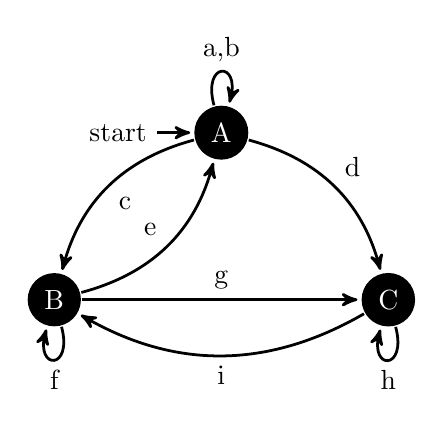
\begin{tikzpicture}[->,>=stealth',shorten >=1pt,auto,node distance=3cm,thick, line width = 1pt]
  \tikzstyle{every state}=[fill=black,draw=none,text=white,minimum size = 0.4cm]

{\node[state,initial]	(A)			{A};}
  
{\node[state]		(B) [below left of=A] 	{B};}
  
{\node[state]		(C) [below right of=A] 	{C};}


\path	(A) edge  [loop above] 	node {a,b} (A)
            edge  [bend right]	node {c} (B)
	    edge  [bend left]	node {d} (C)

        (B) edge [loop below] 	node {f} (B)
	    edge 		node {g} (C)
	    edge [bend right]	node {e} (A)
	
	(C) edge [loop below] 	node {h} (C)
	    edge [bend left] 	node {i} (B)
% 	    edge [bend left]	node {f} (A)
	 ;            
\end{tikzpicture}

%
%\caption{asdfadfs}


\caption{Robot that does a DFS on binary trees.}
\label{fig:dfs}
%\hfill
%\begin{minipage}[b]{0.45\linewidth}
%    \centering
%    \input{butterfly}
%    \caption{}
%    \label{fig: butterfly}
%\end{minipage}
%
%\begin{minipage}[b]{0.45\linewidth}
%    \centering
%    \input{eye}
%    \caption{}
%    \label{fig: eye}
%\end{minipage}
\end{figure}


\paragraph{Configurations and Runs}
A robot walks about a $\Sigma$-graph $G$. Let $R = (Q,\delta)$ be a robot with instruction set $\ins_{\Sigma,1}$. A {\em configuration} $c$ of $R$ on  $G$ is a pair $\tpl{ {v}, {q}} \in V \times Q$. Say that the configuration $\tpl{v,q}$ has {\em position} $v$. A configuration is {\em initial} (resp. {\em halting, repeating}) if $q$ is. The following definition expresses that one configuration results from another after the robot executes a single instruction: for configurations $c = \tpl{v,p}$ and $d = \tpl{w,q}$, say that {\em $d$ results from $c$} iff there is a transition $(p,ins,q)$ of $\delta$ such that $(v,w) \in [[ins]]_G$. 
A {\em run} $\alpha$ of $R$ on $G$ starting with an initial configuration $c$ is an infinite sequence $c_1 c_2 c_3 \cdots$ of configurations  such that $c_1 = c$ and for all $i$, $c_{i+1}$ results from $c_i$.


%Since $R$ is deterministic,  for every configuration $c$ on $G$, there is exactly one run on $G$ starting with $c$. Thus, {\em the run} of $R$ on an initialised graph $(G,v)$ (here $v$ is the initial vertex) is the run starting with configuration $\tpl{v,\iota_Q}$.\sr{Wrong, unless assume regular graph with unique edge labels}

 The {\em set of positions of a run} $\alpha = (v_1,q_1) (v_2,q_2) \cdots $ is the set of positions $\{v_1,v_2,\cdots\}$ of its configurations. The {\em sequence of positions of a run} $\alpha$ is the sequence of positions $v_1 v_2 \cdots$ of its configurations. 
 %The set of directives $\dir$ (that depends on $\Delta$ and $k$) is the set of all operations and all tests, where 
%an {\em operation} is an expression of the form $\go_{i,j}$ for $i,j \in [\Delta]$, and 
%a {\em test} is an expression, or its negation, of the form $\deg_i$ for $i \in [\Delta]$, or
%of the form $\collide_j$ for $j \in [k]$.
%
%A {\em deterministic robot protocol} is a regular language $L \subset \dir^*$ of directives such that every word $w \in L$  $. It is {\em deterministic

\paragraph{Multi-Robot Systems} We now extend the previous definitions to $k$-many of robots.  
%A {\em $k$-initialised graph} is a graph $(G,\tup{v})$ with a $k$-tuple of vertices, called the {\em initial vertices}. 

A {\em $k$-robot ensemble} is a sequence $\tpl{R_1, \cdots, R_k}$ where, writing $R_i = (Q_i,\delta_i)$, each $Q_i$ is a finite set of {\em states}, and each $\delta_i \subset Q_i \times \ins_{\Sigma,k} \times Q_i$ is a finite {\em transition} relation, where the {\em instruction set} is $\ins_{\Sigma,k} :=  \{\uparrow_\sigma : \sigma \in \Sigma\} \cup \msol_k(\Sigma)$.
%, possibly  with initial state $\iota_i$, accepting states $A_i$, and halting states $H_i$.
For a sequence $ins \in ((\ins_{\Sigma,k})^k)^*$ define\footnote{To improve readability, the notation $[[\phantom{n}]]_G$ does not mention $k$.}
  $[[ins]]_G \subseteq V^{2k}$ such that $(\tup{u},\tup{v}) \in [[ins]]_G$ if and only if, in $G$, one can reach $\tup{v}$ from $\tup{u}$ by following the instructions in $ins$.
  
 Formally,
  \begin{enumerate}
  \item If $ins = \epsilon$, then $(\tup{u},\tup{v}) \in [[ins]]_G$ if and only if $\tup{u} = \tup{v}$;
  \item If $ins = (d_1,\cdots,d_k) \in \ins_{\Sigma,k}$
  then $(\tup{u},\tup{v}) \in [[ins]]_G$ if, for each $i \leq k$:%\footnote{This is where we introduce the assumption that robots act {\em synchronously}.}
  \begin{enumerate}
  \item if $d_i = \uparrow_\sigma$ then $\lambda(u_i,v_i) = \sigma$,
  \item if $d_i = \tau(x_1,\cdots,x_k)$ then $u_i = v_i$ and $G \models \tau(u_1,\cdots,u_k)$.
  \end{enumerate}
  \item If $ins = d \cdot e$ then $(\tup{u},\tup{v}) \in [[ins]]_G$ if and only if there exists $\tup{z} \in V$ such that $(\tup{u},\tup{z}) \in [[d]]_G$ and $(\tup{z},\tup{v}) \in [[e]]_G$.

%  $[[ins]]_G := [[d]]_G \circ [[e]]_G$ (where $\circ$ denotes composition of relations).
\end{enumerate}

Fix a $\Sigma$-graph $G$. A {\em configuration} $c$ of $\tpl{R_1, \cdots, R_k}$ on graph $G$ is a pair $\tpl{\tup{v},\tup{q}} \in V^k \times \prod_{i \leq k} Q_i$. A configuration is {\em initial} if $q_i$ is the initial state of robot $R_i$ (for all $i \leq k$). The following definition expresses that one configuration results from another after the robots simultaneously execute their own next instruction (which may be to move along an edge labeled $\sigma$, or to test the current position of all the robots):\footnote{This is where we model the assumption that robots act {\em synchronously}.} configuration {\em $\tpl{\tup{w},\tup{q}}$ results from $\tpl{\tup{v},\tup{p}}$} iff there are transitions $(p_i,ins_i,q_i) \in \delta_i$ (for $i \leq k$) such that $(\tup{v},\tup{w}) \in [[(ins_1,\cdots,ins_k)]]_G$. {\em Runs} and their {\em sets of positions and sequences} are defined as before.
%Since every robot in an ensemble is deterministic, there is a unique run in every initialised graph $(G,\tup{v})$ that starts with the configuration $\tpl{\tup{v},\tup{q}}$ where $\tup{v}$ are the initial vertices of $G$ and $q_i$ is the initial state of robot $R_i$ (for $i \leq k$). 

\paragraph{Robot Tasks} \label{ex:tasks}

Robots should achieve some task in their environment: a {\em $k$-robot task}, or simply a {\em task}, $\T$, is a function that maps a graph $G$ to a set of sequences of positions of $G$, i.e.,  $\T(G) \subseteq (V^k)^\omega$. A robot-ensemble $\tup{R}$ {\em achieves} $\T$ on $G$ if for every run $\alpha$ of $\tup{R}$ on $G$ it holds that $\alpha' \in \T(G)$, where $\alpha'$ is the sequence of positions of the run $\alpha$.
%\sr{should define tasks to be properties of runs? i.e., include states}

We give some examples of foundational robot tasks \cite{KKR07handbook}:
%\sr{cite !!! show foundational}

\begin{enumerate}
\item[RT1.] A robot {\em explores and halts} if, no matter where it starts, it a) eventually halts, and b) visits every vertex of the graph at least once. 
%Formally, $v_1 v_2 \cdots \in T(G)$ if and only if there exists $i$ such that $\{v_1,\cdots,v_i\} = V$ and for all $j \geq i$, $v_i = v_j$.
%\sr{but the robot does not know it halts. tasks should also talk about the sequence of states, not just sequence of positions?}
\item[RT2.] A robot {\em perpetually explores} if, no matter where it starts, it visits every vertex of $G$ infinitely often.
\item[RT3.] A robot {\em explores and returns} if, no matter where it starts, it a) eventually stops where it started, and b) visits every vertex of the graph at least once.
\item[RT4.] An ensemble of robots {\em collaboratively explores} a graph if, no matter where they start, every node is eventually visited by at least one robot.
\item[RT5.] A $k$-robot ensemble {\em gathers} if, no matter where each robot starts, there is a vertex $z$, such that eventually every robot is in $z$.
%Formally, $\tup{v}_1\tup{v}_2 \cdots \in T(G)$ if and only if there exists $z \in V$ and $i \in \nat$ such that for all $j \geq i$,  $\tup{v}_j = (z,\cdots,z)$.

%\item[RT6.] An ensemble {\em decontaminates} a graph if, if every edge is eventually `cleared' (an edge is cleared if there is a robot at each end), and from some point on no cleared edge is `recontaminated' (an edge is recontaminated if there is a robot-free path between that edge and a contaminated edge).\sr{this dfn causes confusion. should it be 'clear' not 'cleared'? possible that all edges are eventually cleared, but that from some point on they are also all contaminated.}
\end{enumerate}



\section{Reasoning about Robot Systems}

We formalise the parameterised verification problem for robot protocols, and then describe our solution to it (Theorem~\ref{thm:PVPdec}) which shows how to reduce parameterised verification in the case of a single robot to the logical validity problem of certain logics.

\subsection{The Parameterised Verification Problem}

The parameterised verification problem depends on a set of graphs $\gclass$, a set of robot ensembles $\rclass$, and a robot task $T$.  Note that $\gclass$ is typically infinite.

\begin{dfn}
The \textbf{parameterised verification problem} $\PVP_\T(\gclass,\rclass)$ states: given a robot ensemble $\tup{R}$ from $\rclass$, decide whether or not $\tup{R}$ achieves the task $\T$ on every graph $G \in \gclass$. 
\end{dfn}

Unfortunately, this problem is easily undecidable for the types of systems we have:
\begin{thm} \label{thm:undec}
There exists a task $\T$ and computable sets $\gclass$ and $\rclass$ such that $\PVP_\T(\gclass,\rclass)$ is undecidable. 

In particular, we can choose $k=1$, $\T$ to be the task ``never halt'', $\gclass$ to be the set of unlabeled-grids, and $\rclass$ to be all robots; or we can choose $k=2$, $\T$ to be the task ``no robot ever halts'', $\gclass$ to be the set of unlabeled-lines, and $\rclass$ to be all robots. 
\end{thm}
%\sr{robots can be taken deterministic}

\begin{proof}[Sketch]
Since the proof technique is a standard, we merely sketch it.  
We reduce the non-halting problem for (Turing-powerful) two-counter machines to $\PVP_\T(\gclass,\rclass)$, i.e., given machine $M$ build robot(s) $\tup{R}$ such that $M$ accepts no input if and only if $\tup{R}$ achieves task $\T$ on all graphs in $\gclass$.

Case $k=1$: As observed by \cite{BlHe67} for their ``2-dimensional automata'', one robot on a grid can simulate two-counter machines: counter values $(n,m) \in \nat^2$ are encoded by the robot being at position $(n,m)$ of the grid. The only tests that are needed are to check whether or not the robot is on the boundary. 
%given a turing machine $M$, build a robot $R_M$ that runs on a grid and checks whether or not the labelings of each row are $M$-configurations that form, in sequence, an accepting run of $M$; if not, then let $R_M$ halt, and otherwise let it run forever. Then $M$ has no accepting run if and only if $R_M$ achieves $T$ on all graphs $G \in \gclass$.

Case $k=2$: The idea is that two distinguishable robots on a line can simulate one robot on a square grid; the position of the $i$th robot on the line gives the $i$th co-ordinate of the single robot on the grid. The robots only need to be able to test if they are at the end points of the line. Alternatively, one can directly code computions of Turing machines, as was done by~\cite{Ro66} to show that universality of $2$-head one-way finite-state automata is undecidable.
\end{proof}

In light of this negative result, our main task is to understand in what way we can restrict the systems to get decidability. 


\subsection{Reducing parameterised verification to validity} \label{subsec:reduc}
%As expected, there is a tradeoff between the various modeling choices. 
%This will involve restricting the combination of $k, \T,\gclass$ and (the testing abilities of robots in) $\rclass$.
We first describe, at a high level, the approach we use to solve (restricted cases of) the parameterised verification problem $\PVP_\T(\gclass,\rclass)$.
Suppose we can build, for every $k$-ensemble $\tup{R}$ of robots, a formula $\phi_{\tup{R},\T}$ such that for all graphs $G$ the following are equivalent:
\begin{itemize}
\item $G \models \phi_{\tup{R},\T}$
\item $\tup{R}$ achieves task $\T$ on $G$. 
\end{itemize}
Then, for every $\rclass$ and $\gclass$, we would have reduced the parameterised verification problem $\PVP_\T(\gclass,\rclass)$ to the $\Phi_{\tup{R},\T}$-validity problem for $\gclass$ where $\Phi_{\tup{R},\T}$ is the set of formulas $\{\phi_{\tup{R},\T} : \tup{R} \in \rclass\}$.\footnote{Note that in our approach $\phi_{\tup{R},T}$ does not depend on $\rclass$ or on $\gclass$.} 
%The {\em validity problem} for a set of formulas $\Phi$ (in the signature of graphs) is to decide, given $\phi \in \Phi$, whether or not every graph satisfies $\phi$.

We now detail this approach in the case of a single robot, i.e., $k=1$.

%
\begin{lem} \label{lem:msodefinable}
Let $R = (Q,\delta)$ be a robot over instruction set $\ins_{\Sigma,1}$, and let ${p}, {q} \in Q$.

We can build $\msol(\Sigma)$ formulas $\psi_{{R},{p},{q}}(X,x,y)$ so that for every graph $G$:
$G \models \psi_{{R},{p},{q}}({X},{x},{y})$ if and only if there exists a run of ${R}$ on $G$ starting from configuration $\tpl{{x},{p}}$ that has a prefix that reaches the configuration $\tpl{{y},{q}}$ and the set of positions on the prefix is exactly $X$.

We can build $\msol(\Sigma)$ formulas $\psi^\infty_{{R},{p},{q}}(X,x,y)$ so that for every graph $G$: $G \models \psi^\infty_{{R},{p},{q}}({X},{x},{y})$ if and only if there is a run of ${R}$ on $G$ starting from configuration $\tpl{{x},{p}}$ that reaches the configuration $\tpl{{y},{q}}$ infinitely often and the set of positions on the run is exactly $X$.
\end{lem}
%
\begin{proof}
A robot $R = (Q,\delta)$ is a finite automaton (without initial or final states) over a finite alphabet $Alph$ of instructions, i.e., $Alph \subset \{\uparrow_\sigma : \sigma \in \Sigma\} \cup \msol_1(\Sigma)$. By Kleene's theorem --- which states that every finite-state automaton can be translated into a regular expression --- we can build a regular expression $exp$ (that depends on $R,p,q$) over alphabet $Alph$ for the language of the automaton $R$ with initial state $p$ and final state $q$.

By induction on the structure of regular expressions over alphabet $Alph$ we build $\msol$ formulas:
\begin{itemize}
\item $\varphi_{\emptyset} := \false$
\item $\varphi_{\epsilon}(X,x,y) := x = y \wedge x \in X$
\item $\varphi_{\uparrow_\sigma} (X,x,y) := edg_\sigma(x,y) \wedge x,y \in X$
\item $\varphi_{\tau}(X,x,y) := x = y \wedge \tau(x) \wedge x \in X$
\item $\varphi_{r + s} := \varphi_{r} \vee \varphi_{s}$
\item $\varphi_{r \cdot s}(X,x,y) := \exists z \left[\varphi_{r}(X,x,z) \wedge \varphi_{s}(X,z,y)\right]$
\item $\varphi_{r^*}(X,x,y) := \forall Z [(cl_{\phi_r}(X,Z) \wedge x \in Z) \to y \in Z]$ where 
\[
cl_{\phi}(X,Z) := \forall a,b \left[(a \in Z \wedge \varphi(X,a,b)) \to b \in Z\right].
\]
\end{itemize}

An easy induction shows that $G \models \varphi_r(X,x,y)$ if and only if there is a sequence of instructions $ins \in Alph^*$ accepted by the regular expression $r$ and a path from $x$ to $y$ that follows instructions $ins$, and that only visits vertices in $X$ (but not necessarily all of $X$). Finally, define the $\msol$ formula $\psi_{R,p,q}(X,x,y)$ to state that $\phi_{exp}(X,x,y)$ holds and $X$ is minimal:
$
\phi_{exp}(X,x,y) \wedge \neg \exists Y (\phi_{exp}(Y,x,y) \wedge Y  \subset X).
$
%An easy induction proves that $G \models \psi_{R,p,q}(X,x,y)$ has the promised property.
%if and only if  Indeed: some run of $R$ on $G$ starting from configuration $\tpl{x,p}$ reaches configuration $\tpl{y,q}$, if and only if, there is a sequence of instructions $ins \in (\ins_\Sigma)^*$ satisfying the regular expression $exp(R,p,q)$ such that $(x,y) \in [[ins]]_G$ (this is proved by a simple induction on the length of sequences involved). The latter is equivalent to $G \models \phi_{exp(R,p,q)}(x,y)$ (this is proved by a simple induction on the structure of the regular expression).


Similarly, by a variation of Kleene's Theorem, we can build an $\omega$-regular expression $exp$ over alphabet $Alph$ for the language consisting of all infinite sequences that label infinite paths in $R$ that start in $p$ and see $q$ infinitely often. Then, inductively build $\varphi_{exp}$, as before, with the following additional rule: 
\[
\varphi_{r^\omega} (X,x,y) := 
\exists z \left[ \varphi_{r^*}(X,x,y) \wedge \varphi_r(X,y,z) \wedge \varphi_{r^*}(X,z,y)\right].
\]
As before, define the $\msol$ formula $\psi^\infty_{R,p,q}(X,x,y)$ to state that $X$ is minimal such that $\varphi_{exp}(X,x,y)$ holds.
\end{proof}

The idea of the proof of Lemma~\ref{lem:msodefinable} follows \cite{BlEn97} who built a formula expressing that there is a run starting in configuration $\tpl{{x},{p}}$ that reaches configuration $\tpl{{y},{q}}$. Our Lemma extends this in two ways, i.e., recording the visited states $X$, and expressing that a configuration occurs infinitely often.
% If one does not need the property ``the set of positions on the prefix/run is exactly $X$'' then we can define the corresponding formulas $\psi_{R,p,q}(x,y)$ and $\psi_{R,p,q}^\infty(x,y)$ in $\fotc(\Sigma)$. 
%This was first proved, using the technique of Lemma~\ref{lem:msodefinable}, in \cite{BlEn97} for the formula $\psi_{R,p,q}(x,y)$, which expresses that the run starting in $(p,x)$ reaches $(q,y)$.\sr{give more credit. be generous}

\begin{note} \label{note:lem1}
The case of multiple robots ($k > 1$) is more subtle. For instance, the analogue of Lemma~\ref{lem:msodefinable} does not hold. Indeed, for $k = 2$, let $R_1 = R_2$ be robots that have one state $p$ and that non-deterministically move in every direction. Then the statement ``there is a run of the robots from configuration $\tpl{x_1,x_2,p,p}$ to configuration $\tpl{y_1,y_2,p,p}$'' is equivalent to the statement that the $k$-ary transitive closure of the edge relation in graph $G$ contains the tuple $\tpl{x_1,x_2,y_1,y_2}$. However, the $k$-ary transitive closure is not expressible in $\msol$ (as was pointed out in Example MF5 in Section~\ref{sec:prelim}). %<--- hard coded example
%It is a challenging problem to find natural and useful restrictions on robots which allow the analogue of Lemma~\ref{lem:msodefinable} to go through. 
\end{note}

%BEGIN OLD
\iffalse
We now present a variation for $k > 1$. The argument mimics that in the proof of Lemma~\ref{lem:msodefinable}. However, the use of the transitive-closure operator is problematic because, as we stated in Example~\ref{ex:ktc} in the introduction, the $k$-ary transitive closure of an $\msol$-formula is not, in general, expressible in $\msol$. 
Thus we make the additional assumption that each robot is star-free. 

\begin{lem} \label{lem:kcompile}
Let $\tup{R}$ be a $k$-robot ensemble, and let $\tup{p}, \tup{q} \in \prod Q_i$. Suppose that, for every $i \leq k$, the language of instructions of automaton $R_i$ with initial state $p_i$ and final state $q_i$ is star-free.

We can build $\msol(\Sigma)$ formulas $\psi_{\tup{R},\tup{p},\tup{q}}$ so that for every graph $G$:
$G \models \psi_{\tup{R},\tup{p},\tup{q}}(\tup{X},\tup{x},\tup{y})$ if and only if the run of $\tup{R}$ on $G$ starting from configuration $\tpl{\tup{x},\tup{p}}$ has a prefix that reaches configuration $\tpl{\tup{y},\tup{q}}$ and the set of positions on the prefix of robot $i$ is exactly $X_i$ (for $i \leq k$).

We can build $\msol(\Sigma)$ formulas $\psi^\infty_{\tup{R},\tup{p},\tup{q}}$ so that for every graph $G$: $G \models \psi_{\tup{R},\tup{p},\tup{q}}(\tup{X},\tup{x},\tup{y})$ if and only if the run of $\tup{R}$ on $G$ starting from configuration $\tpl{\tup{x},\tup{p}}$ reaches configuration $\tpl{\tup{y},\tup{q}}$ infinitely often and the set of positions on the run of robot $i$ is exactly $X_i$ (for $i \leq k$).
\end{lem}
%
\begin{proof}

First build the product automaton $\prod \tup{R}$ over alphabet $Alph \subset (\ins_{\Sigma,k})^k$: the state set $Q$ is $\prod_{i \leq k} Q_i$,  and there is a transition from state $\tup{r}$ to state $\tup{s}$ with label $\tup{d} \in (\ins_{\Sigma,k})^k$ iff $(r_i,d_i,s_i) \in \delta_i$ for each $i \leq k$. We claim that the language of $\prod \tup{R}$ with initial state $\tup{p}$ and final state $\tup{q}$ is star-free. This is an immediate consequence of the following general fact: if $W$ and $W'$ are star-free regular languages over alphabet $B$, then the product language $\{pair(w,w') : |w| = |w'|, w \in W, w' \in W'\}$ is star-free over alphabet $B\times B$, where $pair(w,w')$ is the word $(w_1, w'_1) (w_2,w'_2) \cdots$. To prove this fact use the McNaughton-Papert Theorem and its generalisation to $\omega$-words (discussed in Section~\ref{sec:prelim})  and the simple observation that given $\fol$-formulas $\phi$ defining $W$ and $\phi'$ defining $W'$,  the required $\fol$-sentence defining the product language can be taken as $\phi[P_b \gets \vee_{c\in B} P_{(b,c)}] \wedge \phi'[P_b \gets \vee_{c\in B} P_{(c,b)}]$.

Continue as in the proof of Lemma~\ref{lem:msodefinable}: induct on the star-free $\omega$-regular expression for $\prod \tup{R}$. The Kleene-star and $\omega$-power cases are skipped and we only need deal with the new complementation case. If $r$ is a star-free $\omega$-regular expression then the formula $\varphi_{\neg r}(\tup{X},\tup{x},\tup{y})$ is defined by eliminating negations by repeatedly using the following rules:
\begin{itemize}
\item $\varphi_{\neg \emptyset} := \varphi_{Alph^*}$
\item $\varphi_{\neg \epsilon} := \varphi_{Alph^+}$
\item $\varphi_{\neg \uparrow_\sigma} := $ \sr{FNISH!}
\item $\varphi_{\neg \tau} := \tup{x} = \tup{y} \wedge \neg \tau(\bar{x}) \wedge (\bigwedge_i x_i \in X_i)$.
\item $\phi_{\neg (r + s)} := \phi_{\neg r} \wedge \phi_{\neg s}$
\item $\phi_{\neg (r \cdot s)}(\tup{X},\tup{x},\tup{y})$ is defined as $\exists z. A \vee B \vee C$ where
\begin{align*}
A &:= \phi_{\neg r}(\tup{X},\tup{x},\tup{z}) \wedge \phi_{s}(\tup{X},\tup{z},\tup{y})\\
B &:= \phi_{\neg r}(\tup{X},\tup{x},\tup{z}) \wedge \phi_{\neg s}(\tup{X},\tup{z},\tup{y})\\
C &:= \phi_{r}(\tup{X},\tup{x},\tup{z}) \wedge \phi_{\neg s}(\tup{X},\tup{z},\tup{y}).
\end{align*}
\end{itemize}
One can check that $G \models \varphi_{\neg r}$ if and only if there is a sequence of instructions $ins \in Alph^*$ rejected  by the regular expression $r$ and a path from $\tup{x}$ to $\tup{y}$ that follows instructions $ins$, and that only visits vertices in $\tup{X}$.
\end{proof}
\fi
%END OLD


\subsection{Robot Task Logic --- \RTL} \label{sec:RTL}

We now define a logic, called \RTL, for expressing robot tasks. 

{\bf Syntax.} Formulas of \RTL\ are built, as in the definition of $\msol$ from Section~\ref{dfn:msol}, from the following atomic formulas: $x=y$, $Reach(X,x,y),Halt(X,x,y),Infty(X,x,y)$, and $Rept(X,x,y)$. 


{\bf Semantics.} Formulas of \RTL\ are interpreted with respect to graphs and robots. Thus, given a graph $G$ and a robot $R$ with state set $Q$, initial-state set $I$, repeating-state set $A$, and halting-state set $H$, define the satisfaction relation $\models_\RTL$:
\begin{align*}
\tpl{G,{R}} &\models_\RTL Reach({X},{x},{y}) & \textrm{iff } G \models \bigwedge_{{p} \in I} \bigvee_{{q} \in Q} \psi_{{R},{p},{q}}({X},{x},{y})\\
%
\tpl{G,{R}} &\models_\RTL Halt({X},{x},{y}) & \textrm{iff } G \models \bigwedge_{{p} \in I} \bigvee_{{q} \in H} \psi_{{R},{p},{q}}({X},{x},{y})\\
%
\tpl{G,{R}} &\models_\RTL Infty({X},{x},{y}) & \textrm{iff } G \models \bigwedge_{{p} \in I} \bigvee_{{q} \in Q} \psi^\infty_{{R},{p},{q}}({X},{x},{y})\\
%
\tpl{G,{R}}& \models_\RTL Rept({X},{x},{y}) & \textrm{iff } G \models \bigwedge_{{p} \in I} \bigvee_{{q} \in A} \psi^\infty_{{R},{p},{q}}({X},{x},{y})\\
\end{align*}
The formulas $\psi_{{R},{p},{q}}$ and $\psi^\infty_{{R},{p},{q}}$ are from Lemma~\ref{lem:msodefinable}. Extend the satisfaction relation to all formulas of \RTL\ in the natural way.
%if $k=1$ and Lemma~\ref{lem:kcompile} if $k > 1$; 
%$Q := \prod_{i \leq k} Q_i$ is the set of tuples of states, $I := \prod_{i \leq k} I_i$ is the set of tuples of initial states, $A := \prod_{i \leq k} A_i$ are the repeating tuples, and $H := \prod_{i\leq k} H_i$ are the halting tuples.  We will often supress mention of $k$ and write, for instance, $Reach(\tup{X},\tup{x},\tup{y})$.

%an execution $\alpha \in (V^k \times \prod_{i \leq k} Q_i)^*$ with $\alpha_1$ an initial configuration suppose $I_i \subseteq Q_i$ are the initial states, $A_i \subseteq Q_i$ are the accepting states, and $H_i \subseteq Q_i$ are the halting states:
%$(G,\tup{R}) \models Reach(\tup{x},\tup{y})$ iff there exists a  &\textrm{ iff } \alpha_1 = (\tup{q},\tup{x}) \textrm{ is initial, and } \exists i \in \nat\, \alpha_i = \tup{y}$
{\bf Examples.}
Here are some example \RTL\ formulas and their meanings.
\begin{enumerate}

\item The atomic formula $Reach(X,x,y)$ expresses that the robot, starting in position $x$, reaches position $y$, and the set of visited vertices is $X$.  The \RTL\ formula $\forall x \exists y Reach(V,x,y)$ expresses that the robot explores the graph, no matter where it starts.
%\sr{explain $V$ in MSO formula}

\item The \RTL\ formula $\forall x \exists y Halt(V,x,y)$ expresses ``explore and stop''.

\item The \RTL\ formula $\forall x Halt(V,x,x)$ expresses ``explore and return".

\item The atomic formula $Infty(X,x,y)$ expresses that the robot, starting in position $x$, visits position $y$ infinitely often, and the set of vertices the robot visits along this run is exactly $X$. Thus $\forall x Infty(V,x,x)$ is an \RTL\ formula expressing that the robot ``perpetually explores'' the graph.

%\item The \RTL\ formula $\exists \tup{x} \exists \tup{X} [Halt(\tup{X},\tup{x},\tup{x}) \wedge \cup_i X_i = V ]$, which talks about $k$ robots, expresses that each robot eventually returns and halts in its starting position, and every vertex of the graph is visited by at least one of the robots.
\end{enumerate}

% such and every $k$-robot ensemble $\tup{R} = \tpl{R_1,\cdots,R_k}$, and all $k$-tuples of states $\tup{q},\tup{s} \in \prod_{i \leq k} Q_i$, there is an atomic formula $\tup{R}_{\tup{p},\tup{q}}$  (of arity $2k$) where $\tup{R}_{\tup{p},\tup{q}}(\tup{x},\tup{y})$ expresses that there is an execution of the ensemble $\tup{R}$ starting with configuration $\tpl{\tup{x},\tup{p}}$ and containing\sr{ending?} the configuration $\tpl{\tup{y},\tup{q}}$.

A task $\T$ is {\em captured} by an \RTL\ formula $\vartheta$ if $\tpl{G,{R}} \models_\RTL \vartheta$ is equivalent to the statement that every run of ${R}$ on $G$ is in $\T(G)$.
The example formulas show that the first three tasks from Section~\ref{ex:tasks} are captured by \RTL\ formulas. 

%Formulas written in MSOL can quantify over sets (of vertices and edges). Thus they can express graph properties such as whether the graph is connected, whether it has  a $k$-colouring, whether it is planar, but not whether it is rigid.\sr{are these relevant properties?}

%A cornerstone of automata theory states that MSOL over finite/infinite words/trees coincides with automata operating on finite/infinite words/trees \cite{}. 
%MSOL

Here is the main theorem that solves the parameterised verification problem in the case of a single robot ($k=1$). It reduces the PVP to $\msol$-validity of the set of environments.

\begin{thm} \label{thm:PVPdec}
Fix an edge-label set $\Sigma$. Let $\rclass$ be the set of all robots over $\ins_{\Sigma,1}$,  let $\T$ be a task that is captured by an \RTL\ formula, and let $\gclass$ be a set of $\Sigma$-graphs with decidable $\msol$-validity problem. Then $\PVP_\T(\gclass,\rclass)$ is decidable.
\end{thm}
%
\begin{proof}
Say \RTL\ formula $\vartheta$ captures $\T$. Given ${R} \in \rclass$, build the formula $\phi_{{R},\T}$ by replacing every atomic formula in $\vartheta$ by its definition with respect to ${R}$, e.g., $Reach({X},{x},{y})$ is replaced by $\bigwedge_{{p} \in I} \bigvee_{{q} \in Q} \psi_{{R},{p},{q}}({X},{x},{y})$. A routine induction on the structure of the formula $\vartheta$ gives: $\tpl{G,{R}} \models_\RTL \vartheta$ if and only if $G \models \phi_{{R},\T}$. But by Lemma~\ref{lem:msodefinable} $\phi_{{R},\T}$ is a formula in $\msol(\Sigma)$. Thus we can apply the fact that the $\msol$-validity problem for $\gclass$ is decidable to decide whether or not $G \models \phi_{{R},\T}$ for all $G \in \gclass$.
\end{proof}

%BEGIN OLD
\iffalse
\begin{thm} \label{thm:PVPdec}
Fix $k \in \nat$ and edge-label set $\Sigma$. Let $\rclass$ be the set of all robots over $\ins_{\Sigma,1}$ if $k=1$, and all star-free $k$-robot ensembles over $\ins_{\Sigma,k}$ if $k > 1$. Let $\T$ be a $k$-robot task that is captured by an \RTL\ formula, and let $\gclass$ be a set of $\Sigma$-graphs with decidable $\msol$-validity problem. Then $\PVP_\T(\gclass,\rclass)$ is decidable.
\end{thm}
%
\begin{proof}
Say \RTL\ formula $\vartheta$ captures $\T$. Given $\tup{R} \in \rclass$, build the formula $\phi_{\tup{R},\T}$ by replacing every atomic formula in $\vartheta$ by its definition with respect to $\tup{R}$, e.g., $Reach(\tup{X},\tup{x},\tup{y})$ is replaced by $\bigwedge_{\tup{p} \in I} \bigvee_{\tup{q} \in Q} \psi_{\tup{R},\tup{p},\tup{q}}(\tup{X},\tup{x},\tup{y})$. A routine induction on the structure of the formula $\vartheta$ gives: $\tpl{G,\tup{R}} \models_\RTL \vartheta$ if and only if $G \models \phi_{\tup{R},\T}$. But by Lemma~\ref{lem:msodefinable} (or Lemma~\ref{lem:kcompile} if $k > 1$), $\phi_{\tup{R},\T}$ is a formula in $\msol(\Sigma)$. Thus we can apply the fact that the $\msol$-validity problem for $\gclass$ is decidable to decide whether or not $G \models \phi_{\tup{R},\T}$ for all $G \in \gclass$.
\end{proof}
\fi
%END OLD

%
%\begin{note} \label{note:thm2} Suppose, in Lemma~\ref{lem:kcompile}, one deletes the phrases ``the set of positions on the prefix/run is exactly $X_i$'',  and that test instructions are assumed to be $\mathcal{L}$-formulas, for $\mathcal{L} = \fol(\Sigma)$ or $\mathcal{L} =\fotc(\Sigma)$. Then the promised formulas $\psi_{\tup{R},\tup{p},\tup{q}}(\tup{x},\tup{y})$ and $ \psi_{\tup{R},\tup{p},\tup{q}}^\infty(\tup{x},\tup{y})$ are $\mathcal{L}$-formulas.
%Thus, suppose that $\T$ is definable in the fragment of $\RTL$ that uses these ``set-less'' formulas. If, in addition, all robots are star-free, then to conclude that $\PVP_\T(\gclass,\rclass)$ is decidable, it is enough that $\gclass$ have decidable $\mathcal{L}$-validity problem.
%\end{note}
%

\begin{corollary} \label{cor:CFPVP}
If $\rclass$ and $\T$ are as in Theorem~\ref{thm:PVPdec} and $\gclass$ is a context-free set of graphs, then $\PVP_\T(\gclass,\rclass)$ is decidable.
\end{corollary}

\begin{note} \label{note:dec}
The case of multiple robots ($k > 1$) is harder to analyse. Indeed, Theorem~\ref{thm:undec} states that PVP is undecidable already for $k=2$ on lines (which is a very basic context-free set of graphs) and simple reachability tasks. It is a challenging problem to find natural and useful restrictions on robots which allow the analogue of Corollary~\ref{cor:CFPVP} (or Lemma~\ref{lem:msodefinable}) to hold in the case of multiple robots. 
\end{note}

\section{Illustration: Distributed Computing} \label{sec:DC}

We now instantiate our framework to a popular model of autonomous mobile-agent from the distributed computing literature, i.e., \cite{FIPPP04,Diks200438,Cohen05graphexploration,KKR06,GR08,Das13}. To distinguish their agents from ours, we call theirs {\em DC-robots}.
Here is their model: environments are modeled as undirected graphs, and each vertex is annotated with a local port numbering i.e., for every vertex $v$ the set of labels of the edges of $v$
are in bijection with $\{1,2,\cdots,\deg(v)\}$.  A DC-robot finding itself at vertex $v$ can decide to exit via local port-number $d$ and update its local state based on a) its current state, b) the identification of the robots at the same vertex $v$, c) the degree of $v$, and d) the local-port number of $v$ of the edge it used when arriving at $v$. Thus graphs are assumed to have bounded degree $\Delta$.
Typical tasks from this literature are ``perpetual exploration'', ``exploration with return'', and ``gathering''. The main twist is that the robots should perform their task on a graph no matter the local port numbering. 
%\sr{can relax this and have the edge chosen non-deterministically/fairly amongst those with the same port numbers} 


Such robot systems are easily expressible in our framework. The edge-label set $\Sigma$ is defined to be $[\Delta]$, the edge-relation $E$ is assumed to be symmetric, and $\lambda(v,w) = i$ codes that $i$ is $v$'s port number for the undirected edge $\{v,w\}$. Note that $\lambda(v,w)$ need not equal $\lambda(w,v)$.  The interesting aspect is how to simulate d) above.  Our robot must store in its state both the state of the DC-robot, as well as the local-port number with which it entered the current vertex. It does this as follows: when our robot is at vertex $v$, and the DC-robot says to take exit $i$, our robot first determines the $w$ such that $\lambda(v,w) = i$, and then it determines the $j \in \Delta$ such that $\lambda(w,v) = j$. It can do this with test-instructions in $\fol(\Sigma)$.

{\bf Rotor-Robot} We now give a simple but important example that can be analysed in our framework. The {\em rotor robot} operates as follows: when it enters a vertex $v$ by port $i$ it leaves by port $i+1$ modulo $\deg(v)$. This robot is known by various other names: Abelian mobile robot, rotor walk, ant walk, Eulerian walker, and Propp machine. It is important because it is a viable alternative to probabilistic robots that perform random walks \cite{BL13}. It has the property that it explores all trees --- a result that seems to be folklore, and that could be proved, for fixed degree $\Delta$, using Theorem~\ref{thm:PVPdec}.

{\bf Label-Guided Tasks.}
The graphs in this paper are edge-labeled, but our results hold allowing vertex-labels. Moreover, our framework can incorporate questions of the form: given a robot and a task, decide if for every graph $G \in \gclass$ there exists a labeling of $G$ such that the robot achieves the task on the graph with the help of the labeling. For instance, although there is no DC-robot that perpetually explores all graphs, there is a DC-robot and an algorithm that colours vertices by three colours, such that the robot can perpetually explore every such coloured graph~\cite{Cohen05graphexploration}. Since the set of all graphs does not have decidable-validity, we might only hope to verify variations of this fact for restricted classes of graphs, e.g., fix a context-free set of graphs $\gclass$; then one can decide, given a DC-robot, whether or not for every $G \in \gclass$ the robot achieves the task ``there is a colouring of $G$ using three colours that the robot can use to perpetually explore $G$''. The reason this fits into Theorem~\ref{thm:PVPdec} is that this task is captured by an \RTL\ formula --- indeed, the property that $X_1,X_2,X_3 \subseteq V$ colour a graph is easily expressed in $\msol$ (just say that $\wedge_{i\neq j} X_i \cap X_j = \emptyset$ and $X_1 \cup X_2 \cup X_3 = V$).

%The {\em $r$-DFS robot} operates as follows (for $r \in \mathbb{N}$): it does a depth-first search up to depth $r$ by storing, in its state, the sequence of port numbers leading back to the starting node. This robot perpetually explores all (of the finitely many) graphs of max degree $\Delta$ and diameter $r$ --- it has $\Delta^r$ states, and this is optimal \cite{Cohen05graphexploration}. 
% \sr{connection with Delzanno?}

%For $k \geq 2$, the {\em $(k-1)$-cops and robber game} operates as follows. A single robot plays the robber, and moves at odd time steps; all the remaining $k-1$ robots play cops, and move at even time steps. \sr{complete}


%\item For every $\Delta \geq 2$, there is no robot that perpetually explores all planar graphs of degree at most $\Delta$ \cite{Cohen05graphexploration}.
%
%\item For every $\Delta$, there exist two cop-robots that capture every robber-robot on every tree of degree at most $\Delta$.
%\end{enumerate}


%\begin{enumerate}
%\item Rotor searches trees
%\item $2$-searchers find a visible fugitive on all trees (need the ability to 'see'); or guarding game; ... many variations of evasion-pursuit games.
%\end{enumerate}

%We may encode a $\Delta$-ary tree $T$ with a local port numbering $\pn$ by the $\Bij$-labeled tree $T$, where $\Bij$ is the set of bijections $f:\Delta \to \Delta$, by pushing the numbering into the label.





\section{Complexity Considerations}

%We discuss some limitations of the framework.
%  We have seen (in Theorem~\ref{thm:undec}) that the PVP for our systems may be undecidable. On the other hand, we have also seen restricted classes of systems for which PVP is decidable (Theorem~\ref{thm:PVPdec}).
%\paragraph{High Computational Complexity}
As discussed at the start of Section~\ref{subsec:reduc}, the framework reduces the parameterised verification problem $\PVP_\T(\gclass,\rclass)$ to the $\Phi_{\tup{R},\T}$-validity problem for $\gclass$ where $\Phi_{\tup{R},\T}$ is the set of formulas $\{\phi_{\tup{R},\T} : \tup{R} \in \rclass\}$. Unfortunately, the complexity of the decision procedure in Corollary~\ref{cor:CFPVP} for $\PVP_\T(\gclass,\rclass)$ may be non-elementary, i.e., not bounded by any tower of exponentials in the size of the input robot $R$, even taking $\gclass$ to be the set of binary-labeled lines and $\T$ to be a fixed non-trivial but simple \RTL\ formula such as ``eventually halt''. Indeed: the size of the computed formula $\phi_{R,\T}$ is exponential in the size of the robot $R$ and linear in the size of the \RTL\ formula capturing $\T$, but the complexity of the $\msol$-validity problem for $\gclass$ is non-elementary even taking $\gclass$ to be the set of binary-labeled lines \cite{Stock74}.

Consequently, we illustrate that improved decision procedures can be found for interesting tasks and sets of graphs.
%\sr{what is the complexity for a fixed T and G = words? 
%\sr{prove that there is inherent high complexity}
%\subsection{Overcoming the inherent high computational complexity}
%\sr{discuss undecidability!}
%
%
%

A robot is {\em deterministic} if for all $p \in Q$, either a)  there exists $q,q' \in Q$ and $\tau \in \msol(\Sigma)$ and the only transitions out of $p$ are $(p,\tau,q)$ and $(p,\neg \tau,q')$, or b) there exists $\sigma \in \Sigma, q,q' \in Q$ and the only transitions out of $p$ are $(p,\uparrow_\sigma,q)$ and $(p,\neg \exists z (edg_\sigma(x,z)),q')$. In other words, a) says that if test $\tau$ holds goto state $q$ else goto state $q'$, and b) says that if there is an edge in the graph labeled $\sigma$ then traverse it (in case of many such edges, pick one nondeterministically) and go to state $q$, otherwise goto state $q'$. 
A $\Sigma$-graph is {\em deterministic} if $\lambda(v,w) = \lambda(v,w')$ implies $w = w'$. For instance, $\Delta$-ary trees are deterministic. Note that deterministic robots have at most one run on deterministic graphs.

\begin{thm}  \label{thm:exptime}
Fix $\Delta \in \nat$. Let $\gclass$ be the $\Delta$-ary trees, let $\rclass$ be all deterministic robots, and let $\T$  be the ``explore and halt'' task. Then $\PVP_\T(\gclass,\rclass)$ is \exptimeC. 
\end{thm}

%\sr{basically quantifier free tests are needed.} 

\begin{proof}[Sketch]
The idea is to inter-reduce the parameterised verification problem with the universality problem for deterministic tree-walking automata (DTWA). 
A DTWA is a deterministic machine that can recognise sets of trees: the automaton starts at the root, at any given time the automaton sits on a node of the input tree, can test if the current node is a leaf, the root, or the $i$th child (for $i \leq \Delta$), and based on these tests the machine updates its internal state and executes one of the commands: ``accept the tree", ``reject the tree", ``go to the parent" or ``go the $i$th child".
The universality of DTWA is \exptimeC.
%(this can be deduced from standard facts about DTWA, i.e., emptiness of DTWA is $\exptimeC$,  and complementing DTWA can be achieved by swapping accept and reject states, see \cite{MML06}).
Indeed, from a DTWA $A$ build a DTWA $B$ that simulates $A$ and rejects whenever $A$ runs forever (this causes a quadratic blowup in the number of states \cite{MML06}); then complement $B$ by swapping accept and reject states to get a DTWA $C$; then convert $C$ into an ordinary frontier-to-root tree automaton $D$ using a subset construction that calculates loops of $C$~\cite[Fact $1$]{Boja08} (this causes an exponential blowup); then test $D$ for emptiness (which can be done in \ptime).

Here is the reduction that gives the upper bound: given a deterministic robot $R$ build a DTWA $A_R$ that operates on trees $t$ with marked nodes $s$ and $v$, written $(t,s,v)$, as follows: first it does a DFS from the root, and when it reaches $s$ it begins the simulation of $R$; after the simulation begins, $A_R$ remembers if $v$ is visited; if $R$ enters a halt state and $v$ was visited then $A_R$ accepts $(t,s,v)$, and if $R$ enters a halt state and $v$ was not visited then $A_R$ rejects input $(t,s,v)$. Thus: $R$ ``explores and halts'' iff for all $(t,s,v)$ the run of $R$ on $t$ starting at $s$ visits $v$ and later enters a halt state iff $A_R$ accepts all inputs of the form $(t,s,v)$. The size of $A_R$ is linear in the size of $R$. 

Here is the reduction that gives the lower bound: given a DTWA $A$, build a robot $R_A$ which first explores the input tree $t$ (doing, say, a DFS), then simulates $A$ from the root, and halts iff $A$ accepts (thus $R_A$ runs forever if $A$ rejects). Since $R_A$ always explores its input,  $A$ accepts $t$ iff $R_A$ explores and halts on $t$. The size of $R_A$ is linear in the size of $A$.
\end{proof}

% Next, build a DTWA $B_R$ that simulates $A_R$ and rejects whenever $A_R$ runs forever. This causes a quadratic blowup in the number of states \cite{MML06}. %\sr{check original paper gives Deterministic TWA} 
%Complement $B_R$ by swapping accept and reject states to get DTWA $C_R$. 
%% of whether there is a tree $t$ and a node $v$ on $t$ such that the TWA $C_R$ accepts $(t,v)$. 
% Indeed, $R$ explores and halts on every tree $t$ if and only if $A_R$ (and hence $B_R$) accepts every pair $(t,v)$, where $v$ is a node on tree $t$, if and only if $C_R$ rejects every pair $(t,v)$, i.e., $C_R$ is empty.  This completes the reduction.
%\sr{say something about coding robots as TWA, or import techniques from TWA}

%Convert $A_R$ into a DTWA $B_R$ which always halts, i.e., if $A_R$ runs forever, then $B_R$ rejects. %
%Complement $B_R$ to get a DTWA $C_R$ that accepts $(t,x)$ if and only if Convert $B_R$ into a TWA $C_R$ that accepts tree $t$ if and only if $B_R$ accepts all trees of the form $(t,x)$, for $x \in t$.
%
%$\Sigma := \{ok,abort\} \times \Bij$, that accepts exactly those $\Sigma$-labeled trees such that the robot $R$, starting at the root and operating according to the local port numbering encoded by $f$, eventually stops, and along the way does not visit any vertex with a label from $\{abort\} \times \Bij$. If $R$ never stops and only visits vertices with labels from $\{ok\} \times \Bij$ then the TWA $A_R$ will also run forever. The number of states in TWA $A_R$ is linear in the size of $R$.
%
%
%	Convert $B_R$ into a TWA $C_R$ that first runs $B_R$ to see whether it halts in an accepting or rejecting state. If $B_R$ accepts then $C_R$ runs a DFS from the root to ensure that no vertex is labeled by $\{abort\} \times \Bij$. And if $B_R$ rejects then $C_R$ runs a DFS from the root to ensure that some vertex is labeled by $\{abort\} \times \Bij$. Thus $C_R$ accepts a tree $t$ if and only if either a) $B_R$ accepts $t$ and no vertex of $t$ is labeled by $\{abort\} \times \Bij$, or b) $B_R$ rejects $t$ and some vertex of $t$ is labeled by $\{abort\} \times \Bij$. In the first case the robot $R$ does not explore all of $t$ (it does not reach the node labeled  $\{abort\} \times \Bij$), and in the second the robot $R$first case $t$ is a tree on which the robot $R$
%
%	Thus $C_R$ is empty if and only if robot $R$ explores and stops on all trees. Emptiness of TWA can be solved in EXPTIME \cite{Boja08}.

\begin{note}
For every $\Delta \geq 2$, there is no robot that ``explores and halts'' on all local port-numbered $\Delta$-ary trees \cite{Diks200438}.
The proof above is easily adapted to yield an algorithm that, given a robot $R$ and $\Delta \geq 2$, returns a local-port numbered tree on which the robot does not succeed to ``explore and halt''.
\end{note}

 
%  A weaker model has $k$ many pebbles which the robot can drop and retrieve at vertices. One may further require that a robot can only retrieve the last pebble it dropped (nested pebbles, see \cite{}). %in map making one stores for each vertex the direction to leave.

%The unrestricted whiteboard model on line-like graphs can simulate Turing machines:

%\begin{thm}[whiteboards] \label{thm:wb_undec}
%The parameterised verification problem for a robot with $1$-bit whiteboards on rings and with safety tasks is undecidable, in fact co-re complete.
%\end{thm}

%{\bf Different robots, with individual tasks, that compete.}

%{\bf Faulty Robots.}
%One can allow some fraction of the robots to be faulty, e.g., that it does not comply with the protocol and behaves arbitrarily.\sr{this requires NONDET}

%{\bf Asynchronous model.}
%We can require that at every time step, exactly one robot is non-deterministically chosen to make a move. Moreover, we may require that the schedule is fair \sr{expand,,,, diff notions of fairness}.

%Achieving this aim would give techniques to automatically verify a robot protocol for {\em arbitrary values of the graph parameter(s)}. This would lay the foundation for tools which could i) automatically verify existing theorems whose hand-written proofs are error prone and often ad hoc, ii) facilitate computer-aided experimentation in the theory of RAG.






%\begin{enumerate}
%\item One might define robots independently of $\Delta$: if a robot enters vertex $v$ by port $d$ and is in state $q$ then it leaves via port $(d+f(q,d,deg(v))) \mod deg(v)$ for some fixed $f:Q \times \mathbb{N} \times \mathbb{N} \to \mathbb{N}$.
%\end{enumerate}




%\sr{what about a fixed task? what about a fixed robot?}
%
%
%\section{Discussion}

%Consider the case of robots without whiteboards. We have seen that main limitation of the robot-as-token paradigm is that  we need some form of fairness assumption (such as drunk-robots), and the main limitation of the robot-and-task-as-formula paradigm is that the algorithms are not implementable.



\section{Comparison with Related work} \label{sec:related}

Robot systems are considered distributed if they involve autonomous agents with no central control. In light of this, we first describe the relationship of our work to formal verification of distributed systems generally, and then to formal verification of robot protocols in particular.

\paragraph{Formal verification of distributed systems}
%\vspace{-3.4mm}
Typical parameters that arise in the study of distributed systems are the number of agents, the number of assumed faulty agents, etc. Since parameterised problems of distributed systems are, in general, undecidable~\cite{AK86, Suzuki}, the formal methods community developed sound but incomplete methods that require human intervention, e.g., counter- and predicate-abstractions, inductive invariants, regular model checking and acceleration techniques. See for instance~\cite[references on pages 2-3]{PXZ02}.

On the other hand, by simplifying the systems one can get decidable PVP. These use techniques from games, automata theory and logic, notably finite-model properties/cutoffs, reduction to Petri nets, and the theory of well-structured transition systems~\cite{EN95,EsparzaFM99,EmersonK03LICS,CTTV04,KoLo13AAMAS,Delz14,AJKR14,AKRSV14}. 

Of all these models, token-passing systems (i.e., the models in \cite{EN95,CTTV04,AJKR14,AKRSV14}) are the closest to robots --- both tokens and robots move along the vertices of graphs. However, we now argue that the model in these cited papers is incomparable with our model. First, the translation of their token-passing systems into robot systems would require that robots can read and write to variables at the vertices (this is to model the fact that processes have states). However, we assumed environments are static (because otherwise the PVP is quickly undecidable). Conversely, translating robot-systems into the cited token-passing systems requires that the robot-systems satisfy the following unrealistic assumptions (that are used in their decidability proofs): when a robot decides to move, an adversary decides which edge it takes, as well as to which of its internal states to transition (i.e., even the robot's memory may be scrambled). Not even the simplest robots from the distributed computing literature (e.g., the rotor robot, or the DFS robot)  satisfy this double restriction.

\paragraph{Formal verification of robot systems}
The formal methods community has only recently \cite{HMM11,Devi11,Bonnet12,Berard13,ABCTU13,MPST14} begun explictly verifying and synthesising robot protocols (rather than distributed systems in general). However, half of these papers only treat small values of the parameters.  For instance, one such paper concludes \cite[page 11]{Berard13}: 

\begin{quotation}
{\it While our method is parameterised by both k [the number of robots] and n [the size of the graph],
it does not permit to verify 
whether a [robot] protocol is valid for every k and n satisfying a particular predicate. 
}
\end{quotation}

The papers that do treat parameterised robot protocols do not give sound and complete decision procedures for their systems, as we do. Indeed, \cite{ABCTU13} uses a proof assistant to provide certificates (formal proofs) of impossibility results about robot networks; \cite{MPST14} uses the theory of games on graphs to synthesise a robot protocol for gathering $k$ robots on a ring of size $n$ (for small values of $k,n$), and relies on a hand-proven induction to prove that the synthesised robot protocol works for all values of the parameters $k,n$; and \cite{KoLo15} presents a sound technique that may identify cutoffs using a counter-abstraction in order to draw conclusions about certain swarm algorithms, independently of the number of swarming agents.
%\sr{mention Allessio's work? they DO PV, but is it robots really?}

The quotation above continues:
\begin{quotation}
{\it Adapting recent advances in parameterised model checking [citation elided] would be a nice way 
to obtain such results. }
\end{quotation}

Both the methodology (reducing parameterised verification of robot systems to validity problems in logic) and the results of this paper (algorithms for automatic parameterised verification of robot systems consisting of a single robot in an unknown environment) are novel and have succeeded where other methods and ``recent advances'' (discussed in the previous subsection) have not.  

%Indeed, as discussed in the previous subsection, recent advances in parameterised model checking were not used in this paper; rather, this paper presents a novel approach based on standard automata theory. 
%
%{\it $2.$ Our approach aids in the design of mobile robot protocols by permitting 
%to find bugs and loopholes in the overall logic. Going one step further and 
%generating the protocol automatically from the problem would permit to get 
%solutions that are correct by design. We believe that controller synthesis [citation elided]
%can be extended to obtain such guarantees.} 
%

%The novelty of the framework we suggest is that it allows {\em automatic} verification. 

%Of course, the drawback of using completely automatic techniques, is that the types of robots and tasks that can be dealt with are, necessarily, more limited than those appearing in the theoretical literature. However, this work gives a much clearer understanding of the border between classes of robot protocols that can be automatically verified, and those that cannot.

\paragraph{Comparison with graph-walking automata}
%
{\bf Graph-walking automata.} There is no canonical definition of automaton on graphs. Our model of a single robot is equivalent to graph-walking automata with $\msol$-tests~\cite{BlEn97}. The proof idea of Lemma~\ref{lem:msodefinable} (which compiles robots into formulas over graphs) is borrowed from \cite{BlEn97, EnHo06}. Other classical notions of automata on graphs (e.g., \cite{BlHe67}) are often too expressive and lead to undecidable parameterised verification problems (see the proof of Theorem~\ref{thm:undec}). 


{\bf Multi-head automata.} If agents are modeled as finite-state machines, then multi-agent systems are instances of multi-head automata, and the parameterised verification problem for reachability tasks is equivalent to the universality problem for such automata.  A technical difference between our robot-ensembles and multi-head automata is that the $k$-heads of a multi-head automaton are operated from a central control. In the language of robots this would mean that the robots can communicate their current local states to each other. Such communication is disallowed as it quickly results in undecidability. Unfortunately, Theorem~\ref{thm:undec} shows that, for multiple robots, even simple communication leads to undecidability.

{\bf Tree-walking automata (TWA)} are a natural generalisation to trees of two-way automata on words. Tree-walking automata with a single head, and their corresponding regular expressions, have been studied for their own sake \cite{Boja08}, in formal verification, e.g., \cite{Vardi98,BLMV08,Obdr13}, and as tree pattern-matching tools \cite{BrWo00, Schw12}. TWA are used in Theorem~\ref{thm:exptime} to reason about a single robot on an unknown tree.

%Our definition of robot-ensemble can be viewed as a contribution to the theory of multi-head graph-walking automata with decidable universality problem.

%{\bf Two-way word automata.} For instance, two-way $k$-head word automata are like ordinary word automata except that they have $k$-many heads (instead of one) and each head can move in both directions. In the language of robots, this means that the $k$-many robots operate on labeled lines and  communicate via a central control, i.e., the robots can communicate their current local states to each other. However, the universality (and emptiness) problem for such automata with central control is undecidable for $k > 1$~\cite{}, and decidable for $k=1$ (in fact, every two-way $1$-head automata can be effectively converted into an ordinary word automaton that accepts the same set of words \cite{}).
%However, as we saw in Theorem~\ref{}, this is still not enough to get decidability of the PVP, and so, in the case $k > 1$, we further restricted the robots to be star-free (Section~\ref{}).
%
%They accept just the regular languages, but may be exponentially more succinct than one-way automata \cite{}. 

%
%{\bf Two-way tree automata.}
%Two-way tree automata are like two-way string automata, but they operate on trees (of fixed degree). Thus there is a single head that can recognise if it is at the root, or a leaf, or the $i$th child, and it can move to the parent or to the $j$th child. They recognise a proper subset of the tree-regular languages \cite{}.
%


%Two-way string automata are like ordinary string automata except that they can move the head in both directions. 

%\cite{BlEn97,EnHo06} 



% A $1$-head TWA can be viewed as a robot walking over a tree, with tests of the form ``leaf?'', ``root?'', ``left-child''?, etc. Similar regular expressions of instructions (in the context of trees of arbitrary degree) are called caterpillar expressions in \cite{BrWo00} where they are studied and used as tree-pattern matching tools.

%The classic result in this area is that first-order logic with $k$-ary deterministic\sr{why det?} transitive closure has the same power as $k$-head deterministic tree-walking automata that use a finite set of pebbles (which may be dropped and retreived on vertices in a nested fashion).~\cite{EnHo06,Lucspaper}.
%This result holds for graphs for which perpetual exploration is possible (called ``searchable'' in that paper). 

%The $k$-heads may be thought of as $k$-robots that communicate via central control.


%Although TWA have deep connections to logic (\cite{EnHo06,Lucspaper}) and formal verification (e.g.,\cite{Vardi98,BLMV08,Obdr13}), these connections have not yet been exploited for verification of robot protocols.


%Graph automata operating on grids with marked borders were introduced in \cite{BlHe67}. They can simulate two-counter machines (the $x,y$-coordinate gives the counter content), and thus emptiness (and universality) are undecidable. 
%This means that parameterised verification of reachability tasks for these robots is undecidable.

%For instance, the graph automata of \cite{BlHe67}, which operate on grids with marked borders, can simulate two-counter machines (a model of computation equivalent to Turing machines) since the robot's $x,y$-coordinate may be used to represent counters, and thus the non-halting problem of $2$-counter machines, known to be undecidable, reduces to the parameterised verification of reachability tasks.

%{\bf Multi-head automata.} A $k$-robot ensemble may be viewed as a single graph-walking automaton with $k$-many heads~\cite{EnHo06}. \sr{say more!}

% We now discuss the relationship between robot-ensembles and other notions of graph-walking automata in the theoretical computer science literature.
 
   % Directive automata can be thought of as finite-string automata that accept sequences of directives, i.e., instructions how a robot should move in a graph, and such automata can be compiled into a suitable logical language (MSOL)~\cite{BlEn97}. 
% 


%{\bf Maze-walking automata.}
%A maze is a connected subgraph of a grid. A maze automaton has finite control and can recognise which compass directions in the grid are free and move in those directions and change state. No maze automaton, even with a pebble that it may drop and retrieve, can solve perpetual exploration on every maze \cite{Hoff81}. More maze-exploration references can be found in \cite{szep95}.

%{\bf Directive automata.} An early reference to graph-walking automata is \cite{BlEn97}. These can be thought of as finite-string automata that accept sequences of directives, i.e., instructions how a robot should move in a graph. These automata can be compiled into MSOL, and form the basis of Section~\ref{sec:basicmodel}. 



%\paragraph{Other formalisms like PLDL, Fagin's Interpreted Systems and Temporal logics, etc.}\sr{REWRITE!} 
%
%
%The PLDL and related formalism (STRIPS, event calculus, situation calculus) are based on $\fol$ and are used to express and simulate dynamic domains. However, each environment must be expressed separately.\sr{is this true? is it possible to code 'i am on a ring of some unknown size'?} 
%One innovation of the framework in this paper is that it can express a set of environments (rather than just a single environment). In other words, our framework naturally allows one to explicitely express families of domains (= environment + robot + task). Moreover, our logic for expressing robot tasks, \RTL,  has the ability to quantify over the vertices of the graph, unlike temporal logic which can only access fixed predicates of the graphs.


\section{Future Challenges} \label{sec:future}

%However, there is also a philosophical difference which might explain why this connection has not been exploited before: a robot is supposed to complete some task on the tree, while a TWA accepts or rejects the tree. Thus, from a robot point of view the interesting question is not whether or not the TWA accepts, but rather what the {\em behaviour} of the TWA on its input looks like --- e.g., does the {\em run} of the TWA visit every node of the input tree? 

Here is a general research problem: find other natural robot systems that have decidable or tractable PVP.

Regarding decidability, much work remains to be done. An important problem is to extend the methodology or results of this paper to \underline{multiple} robots. Notes~\ref{note:lem1} and~\ref{note:dec} discuss the challenges facing such an investigation.

Similarly, in light of the fact that PVP is quickly undecidable in a \underline{dynamic environment} (e.g., this is the case for simple reachability tasks of a single robot that can read and write to every vertex on a line, cf. \cite{Suzuki,EN95}), what restrictions on the robot or the dynamic environment will result in decidable PVP? 

On the other hand, we believe it is feasible to extend our framework to \underline{quantitative tasks}, such as minimising the number of steps to complete a task.

%Also, if one extends the robot capabilities to communicate via rendezvous then howto what extent can one change the modeling choices listed in the introduction? The main challenge is to find natural or useful modeling choices with reasonable tradeoffs. For instance,  e.g., PVP is undecidable if one assumes that robots can communicate by rendezvous (e.g., allowing the robots to communicate their local states) on lines or trees (cf. ) but decidable on cliques (cf. ). \sr{remove all conjectures. make vauge statements}
%It is a research topic to vary all of the modeling choices individually or together and look for decidable subcases. AtUnfortunately, the PVP is undecidable if one assumes a dynamic environment instead of a static environment (e.g., allowing the robots to read and write $b \in \nat$ bits at each vertex results in undecidable PVP even for $b=1$, line-graphs, and reachability tasks, cf. \cite{Suzuki}). Also, PVP is undecidable if one assumes that robots can communicate by rendezvous (e.g., allowing the robots to communicate their local states to each other when they are on the same vertex). \sr{CHECK: There is no literature on general formalisms and decidability results dealing with probabilistic robots, continuous environments, asynchronous evolution, or other modes of communication.} 

Regarding complexity, we have seen that our general algorithm  for solving the PVP (in Theorem~\ref{thm:PVPdec}) has high computational complexity, and we have seen (in Theorem~\ref{thm:exptime}) that a certain problem on trees is \exptimeC. For which systems (tasks, classes of graphs, and classes of robots) is the PVP solvable in \ptime, \np, or \pspace? 

%Third, our framework is limited to a fixed number of agents. Can one extend the framework to include the number of agents as a parameter? 
%
We believe that tackling these questions will open avenues both in automata theory and in the verification of mobile multi-agent systems in unknown environments.
%For which context-free sets $\gclass$ is there an elementary decision procedure to decide if a robot ``explores and stops''? What other tasks have elementary decision procedures? 
%
%Synthesis
%
%Quantitative objectives/efficiency: e.g., prove rotor robot cover in ptime.
%
%Open systems
%
%non-finite state robots: e.g., one counter robots. (see blum+kozen)

\section*{Acknowledgements}
I thank the reviewers for their careful reading and provocative questions which helped improve the content and presentation of this paper.

\bibliographystyle{abbrv}
\bibliography{../../MarieCurie/lit-mc}

\end{document}
\newpage


\section{NEXT STEPS}
\begin{enumerate}
\item the phrase  'distributed multi-robot system' is relevant/important.
\item give ROBOT EXAMPLES! to show power of the model! very powerful sensing! but not communication (e.g., broadcast).
\item Mention (in extensions?) that we don't allow absolute distances (such as 	in the 10FPS paper, since procs have constant memory, and graphs are unbounded in size), but we do allow relative positioning (e.g., robot 1 is to my left).
\item PROVE conversion theorem (robot to regexp to formula) for robots which know port number they land in.
\item Is FO + binary TC enough? in which case, which graphs are decidable?
\item cite Alessio early!
\item 'mobile' usually means the netowrk is dynamic. what is the jargon for static env? 
\item 'calc of mobile agents' is a ccs-like coomunication channels and locations. it captures the structure of complex networks and the behavior of mobile computation. 
\item mobile computations  = virtual mobility on static network; mobile computing = moving computers, so dynamic network.
\item say somewhere that logic is used to specify the 'structure'/environment and the tasks (and even the procs).
\item emptiness of graph-automata should be linear/polynomial in the tree-width.
\item DFNs of autonomous etc.: KRR, and Fisher. ``Mobile Agent Computing''
\item Why anonymous? env. might be hostile and so don't have IDs. or there might be faults (see Yu +Yung for short  discussion)
\item Why PMCP? Abstraction for unknown environment, or very large environment.
\item Why is this relevant to AAMAS community? e.g., high level decision part of cyber-physical system. foundations for practical systems, highlighting critical issues. Go through theory papers.
\item Formalise language in which to describe tasks. WHAT EXISTING LANGUAGES ARE THERE? COMPARE! somehow point out that the graph is explicit in this framework, while it is implicit in other scenarios (e.g., agentspeak, METAM)

I am trying to create a logic for reasoning about mobile agents on graphs. All the logics I can find (e.g., PDDL, situation calculus, mu-calculus) require that one codes the graph and the agents in a single system. Do you know any exceptions to this? i.e., a logic L, to be interpreted on graphs G, in which one can express things like 'the robber avoids being caught in the cops-robber game on graph G'.

\item Formalise robot system that are treated. Might want to follow GWA of EnBl97, but for undirected graphs. There each edge has a label from a finite set. This finite set could include both port numbers (and the direction if you want directed graphs).

Idea works for deterministic robots + locally port numbered graphs + synchronous movement, i.e., there is a unique run.
Then: there is a formula $\phi_L(x,y)$ that means the robot moves from $x$ to $y$ along a path whose label set is $L$. Then exploration can be expressed as $\forall x \forall y \phi_{true}(x,y)$.

If movement is asynchronous, then there can be a set of runs. Somehow must express "for all $x$ there is a run $\pi$ starting in $x$ and whose occurence set is $V$".

\item Prove lower bounds!
\item Run experiments using tree-automata packages, or SMT solvers!
\item Decide on generality of statements (e.g., competing robots? different robots?)
\item Bibliography chronological or alphabetical?
\item include discussion of synthesis in intro?
\item stress that the graphs are not arbitrary? i.e., unknown means unknown but in some known class?
\item finish going through pc members' most cited papers and relevant papers to see their interests.
\item future work: can one automatically prove a property independently of $\Delta$?
\item labeling from fixed alphabet allowed?
\item robot logic is linear-like. say something about branching case.
\item say something about asynch case


\item Here is an intuition of how we might use automata and logic to decide the parameterised verification problem for robots without whiteboards. A robot operating on a labeled line can be thought of as a two-way automaton; the labeling of the line is read as a string. The point is that questions about robots on ``linear'' graphs (such as lines or rings), are questions about the runs of two-way automata on strings (e.g., ``does the run visit every position of the string?'' corresponds to perpetual exploration). Similarly there are tree-automata that operate on labeled trees. 

 Although there is no canonical notion of graph-automaton, we can use monadic-second order logic to reason about robots operating on all graphs from a context-free set $\gclass$.

In fact, by Courcelle's Theorem, the parameterised verification problem is decidable if $\gclass$ is a context-free set of graphs.

\end{enumerate}
\end{document}



If robots are deterministic with unique initial states then all the robot tasks introduced in Section~\ref{ex:tasks} are expressible in the fragment of \RTL\ that itself is expressible in $\fotc$. For instance, the ``explore and stop'' task can be expressed as $\forall x [\exists y Reach_f(x,y) \wedge \forall y reach(x,y)]$. Note that if we drop the assumption that robots are deterministic, then this formula does not work (it only guarantees that every vertex is visited by some run, but not necessarily the same run for different vertices).

\begin{enumerate}
\item ``explore and return'' can be expressed as
\[
\forall x [ Reach_f(x,x) \wedge \forall y Reach(x,y)].
\]
\item ``perpetual exploration'' can be expressed as 
\[
\forall x [\neg \exists y Reach_f(x,y) \wedge \forall y Reach(x,y)].
\]

\item ``gathering'' of $k$-many robots can be expressed as
\[
\forall x_1 \cdots \forall x_k \exists y Reach_f(x_1,\cdots,x_k,y,\cdots,y)
\]
\end{enumerate}

\sr{note that MC FOL properties is in PSPACE since the formula in it FOL+DTC.}

\sr{alt dfn}\sr{add atoms?}

A {\em robot protocol} is a tuple

\[
\left< \Delta,k,Q,\iota,T, \update,\exit \right>
\]
where $\Delta \in \nat$ is the {\em graph degree}, $k \in \nat$ is the {\em number of robots}, $Q$ is a finite set of {\em states}, $\iota \in Q$ is the {\em initial state}, $T$ is a set of MSOL formulas called {\em tests}, $ \update:Q \times 2^{[T]} \to Q$ is the {\em state-update function}, and $\exit:Q \times [\Delta] \to [\Delta]$ is the {\em move function} and satisfies $0 \leq \exit(s,d) \leq d$. 

Taking $T = \emptyset$ results in 
A {\em robot protocol} is a tuple
\[
\left<\Delta,k,Q,\iota, \update,\exit\right>
\]
where $\Delta \in \nat$ is the {\em graph-degree}, $k \in \nat$ is the {\em number of robots}, $Q$ is a finite set of {\em states}, $\iota \in Q$ is the {\em initial state}, and writing $D := [\Delta]$, $ \update:Q \times D \times D \times 2^{[k]} \to Q$ is the {\em state-update function}, and $\exit:Q \times D \to D$ is the {\em move function} and satisfies $0 \leq \exit(s,d) \leq d$. 
%It is a {\em finite-state robot} if $Q$ is finite.
% Define functions $\mem, \exit$ by the identity $ \update(q,d,X) = (\mem(q,d,X), \exit(q,d,X))$.

Fix a graph $(V,E,\pn)$. A {\em configuration} is a pair of functions $(v,q)$ where $v : [k] \to V$ and $q : [k] \to Q$. An {\em execution} is a sequence of configurations $(v_0, q_0), (v_1,q_1)  \dots$ %for which there exists a sequence $d_0, d_1, \dots$ of elements of $D$ 
such that for all $i \leq k$ and all $t \geq 0$:
\begin{enumerate}
\item $q_{0}(i) = \iota$, 
\item $v_t (i) \xrightarrow{d_t(i)} v_{t+1}(i)$,
\item $q_{t+1}(i) =  \update(q_t(i),\deg(v_t(i)),p_t(i),s_t(i))$.
\end{enumerate}
where $d_t(i) := \exit(q_t(i),\deg(v_t(i)))$ (i.e., the direction in which robot $i$ moves at time $t$), $p_t(i) := \pn(v_{t+1}(i),v_t(i))$ (i.e., the entry port number of the successive vertex of robot $i$) and $s_t(i) := \{j \leq k : v_t(j) = v_t(i)\}$ (i.e., the set of robots at the same vertex as robot $i$ at time $t$).
%In words, every robot:
%\begin{enumerate}
%\item starts in the initial state,
%\item moves in direction given by the $\exit$ function and depending on its current state and degree of the current vertex it is at,
%\item changes state given by the $ \update$ function and depending on the current state, the degree of the current vertex, the set of robots in the same current vertex, and the local port number of the edge entering the next vertex.
%\end{enumerate}

%In particular, every state (besides, possibly, the initial state) stores the last entry port number.

Say that the execution {\em starts in $v_0$}. Note that $v_0 : [k] \to V$ determines the execution starting in $v_0$ since robots are deterministic. If $(v,q)$ is an element of an execution then we say that robot $i$ of the execution {\em visits vertex $v(i)$} and {\em enters state $q(i)$}.
% In words, a robot in state $q$ and at vertex $v$ changes state to $\mem(q,deg(v))$ and exits via port $\exit(q,deg(v))$. Initially the robot starts in state $\iota$ with direction $1$.\footnote{Some models allow the memory function $\mem$ also to depend on the last direction taken, eg., \cite{FIPPP04}. This does not increase the expressive power since our model can store the last direction taken in the state.}








 
%An {\em graph with local port numbers from $D$} is a triple $(V,E,\pn)$ with $V$ a finite set of {\em vertices}, and $E \subseteq V \times V$ a symmetric {\em edge} relation,  and $\pn:E \to D$, called a {\em local port-numbering}, is an injection when restricted to the edges incident to a vertex, i.e., for every $v \in V$, $\pn$ restricted to $\nhd(v) := \{(v,w) \in V^2: (v,w) \in E\}$ is an injection into the set $D$. If $\pn((v,w)) = d$ then we will write $v \xrightarrow{d} w$. Write $\pn(v)$ for the image of $\pn$ restricted to $\nhd(v)$.


%Formally, a {\em local port numbering} of an undirected graph $(V,E)$ is a function $\pn:E \to [\Delta]$ such that for every $v \in V$, $\pn$ restricted to the edges $\{(v,w) : (v,w) \in E\}$ is  a bijection to $[deg(v)]$. 

%%% DC LIT DFNS OF ROBOT SYSTEMS
%\paragraph{Robot environments}
%A {\em discrete environment} or {\em graph} is a triple $(V,E,\pn)$ with $V$ a finite set of {\em vertices}, and $E \subseteq V \times V$ a symmetric reflexive {\em edge} relation such that $|E(v)| \leq \Delta$ for all $v \in V$ (where $E(v) := \{(v,w) \in V^2: (v,w) \in E\}$), and $\pn:E \to [\Delta]$, called a {\em local port-numbering}, satisfying that for every $v \in V$,  a) $\pn(v,v) = 0$, and b) $\pn$ restricted to $\nhd(v)$ is a bijection onto $[\deg(v)]$. If $\pn(v,w) = d$ then we will write $v \xrightarrow{d} w$. Note that $\pn(v,w)$ need not equal $\pn(w,v)$.
%
%For example, a {\em ring} is a graph $(V,E)$ with $V := [n]$ (for some $n$) and $E := \{(i,i+1) : i \in [n]\}$ (all arithmetic is modulo $n$). It has a local port-numbering so that $i \xrightarrow{0} i$, $i \xrightarrow{1} i+1$ and $i \xrightarrow{2} i-1$.
%
%Another example is a {\em torus} graph $(V,E)$ with $V := [n] \times [n]$ (for some $n$) and local port-numbered edges that $i \xrightarrow{0} i$, $(i,j) \xrightarrow{1} (i,j-1)$, $(i,j) \xrightarrow{2} (i,j+1)$, $(i,j) \xrightarrow{3} (i-1,j)$ and $(i,j) \xrightarrow{4} (i+1,j)$ (arithmetic is modulo $n$).

% One aim of this work is to give a framework in which one can automatically prove such statements.



\subsection{LRT: A Logic for Robot Tasks}


The following variation shows that if we are not interesting in keeping the set of visited vertices in a set $X$, then we can write the formulas in $\fotc$, a fragment of $\msol$.
\begin{lem} \label{lem:fotcdefinable}
Repeat the assumptions in Lemma~\ref{lem:msodefinable}.
We can build $\fotc(\Sigma)$ formulas $\phi_{\tup{R},\tup{p},\tup{q}}$ (and $\phi^\infty_{\tup{R},\tup{p},\tup{q}}$) of $2k$ first-order variables so that, for every graph $G$: $G \models \phi_{\tup{R},\tup{p},\tup{q}}(\tup{x},\tup{y})$ if and only if the run of $\tup{R}$ on $G$ starting from configuration $\tpl{\tup{x},\tup{p}}$ reaches configuration $\tpl{\tup{y},\tup{q}}$ (infinitely often).\sr{There are also formulas non-deterministic robots, with 'some run' and 'for all runs' replacing 'the run'.}
\end{lem}

\begin{proof}
To define the formulas $\phi_{R,p,q}(x,y)$ and $\phi^\infty_{R,p,q}(x,y)$ in $\fotc$, proceed as in Lemma~\ref{lem:msodefinable}: build formula $\varphi_r(x,y)$ as follows:
\begin{itemize}
\item $\varphi_{\emptyset} := \false$; and $\varphi_{\epsilon}(x,y) := x = y$.
\item $\varphi_{\uparrow_\sigma} (x,y) := edg_\sigma(x,y)$.
\item $\varphi_{r + s} := \varphi_{r} \vee \varphi_{s}$; and $\varphi_{\varphi}(x,y) := x = y \wedge \varphi(x)$.

\item $\varphi_{r \cdot s}(x,y) := \exists z [\varphi_{r}(x,z) \wedge \varphi_{s}(z,y)]$.
\item $\varphi_{r^*}(x,y) := \forall Z [closed_{\phi_r}(Z) \wedge x \in Z) \to y \in Z]$.
\item $\varphi_{r^\omega} (x,y) := \exists z [\varphi_{r^*}(x,y) \wedge \varphi_r(y,z) \wedge \varphi_{r^*}(z,y)]$.
\end{itemize}
Then define $\phi_{R,p,q}(x,y)$ as $\varphi_{exp}(x,y)$, and $\phi^\infty_{R,p,q}(x,y)$ as $\varphi^\infty_{exp}(x,y)$, where $exp$ is the regular expression for the language of the automaton $R$ with initial state $p$ and final state $q$.
\end{proof}

%Thus:
%\begin{itemize}
%\item $\varphi_{\emptyset} := \false$.
%\item $\varphi_{\epsilon}(x,y) := x = y$.
%\item $\varphi_{\uparrow_\sigma} (x,y) := edg_\sigma(x,y)$.
%\item $\varphi_{\varphi}(x,y) := x = y \wedge \varphi(x)$.
%\item $\varphi_{r \cdot s}(x,y) := \exists z [\varphi_{r}(x,z) \wedge \varphi_{s}(z,y)]$.
%\item $\varphi_{r + s} := \varphi_{r} \vee \varphi_{s}$.
%\item $\varphi_{r^*} := (\varphi_r)^*$, defined in Section~\ref{ex:formulas}.
%\item $\varphi_{r^\omega} := (\varphi_r)^\omega$, defined in Section~\ref{ex:formulas}.
%\end{itemize}

In order to deal with more classes of graphs $\gclass$, we can restrict tasks to being definable $\RTL'$, a variation of \RTL\ that uses the formulas of Lemma~\ref{lem:fotcdefinable} instead of Lemma~\ref{lem:msodefinable}:
\begin{align*}
\tpl{G,\tup{R}} &\models_\RTL reach(\tup{x},\tup{y}) & \textrm{ iff } G \models \bigwedge_{\tup{p} \in I} \bigvee_{\tup{q} \in Q} \phi_{\tup{R},\tup{p},\tup{q}}(\tup{x},\tup{y})\\
%
\tpl{G,\tup{R}} &\models_\RTL halt(\tup{x},\tup{y}) & \textrm{ iff } G \models \bigwedge_{\tup{p} \in I} \bigvee_{\tup{q} \in H} \phi_{\tup{R},\tup{p},\tup{q}}(\tup{x},\tup{y})\\
%
\tpl{G,\tup{R}} &\models_\RTL infty(\tup{x},\tup{y}) & \textrm{ iff } G \models \bigwedge_{\tup{p} \in I} \bigvee_{\tup{q} \in Q} \phi^\infty_{\tup{R},\tup{p},\tup{q}}(\tup{x},\tup{y})\\
%
\tpl{G,\tup{R}}& \models_\RTL rept(\tup{x},\tup{y}) & \textrm{ iff } G \models \bigwedge_{\tup{p} \in I} \bigvee_{\tup{q} \in A} \phi^\infty_{\tup{R},\tup{p},\tup{q}}(\tup{x},\tup{y})\\
\end{align*}

Then we have
\begin{thm} 
Let $\T$ be a task that is captured by an $\RTL'$-formula, let $\gclass$ be a set of graphs with decidable $\fotc(\Sigma)$-validity problem, and
let $\rclass$ be the set of all deterministic robot ensembles. Then $\PVP_\T(\gclass,\rclass)$ is decidable.
\end{thm}

% Logic can be used to define sets of graphs $\gclass$ as well as sets of tasks $\mathcal{T}$. 



\subsection{Verification Algorithm}

The main idea is to reduce the parameterised verification to the validity (i.e., the complement of satisfiability) of MSOL.

\begin{thm} 
Fix $\gclass$ such that validity of MSOL is decidable on $\gclass$. Then there is an algorithm that solves the parameterised verification problem for the set $\rclass$ of all finite-state robot protocols and the set $\tclass$ of all LRT-definable tasks.
\end{thm}

\begin{proof}
Following \cite{BlEn97,EnHo06} the idea is to % think of the given robot as a graph-walking automaton \cite{BlEn97}. This is then 
compile the robot into an MSOL formula~\footnote{Iin fact, like the graph walking automata of \cite{BlEn97,EnHo06}, a finite-state robot can be compiled into a formula of first-order logic with transitive closure.} $\phi_{p,q}(x,y)$ such that $(G,a,b) \models \phi_{p,q}$ iff the robot starts at vertex $a$ in state $p$ and reaches vertex $b$ in state $q$. This can be done as follows. First, if we think of a robot as a describing sequences of directions, we can take a regular expression for the set of sequences labeling paths from $p$ to $q$. Second, go by induction on the regular expression to build the required formula.

\begin{itemize}
\item Base case:

\item Union: use disjunction

\item Concatenation $L_1 \cdot L_2$ compiles into $\exists v. \phi_1(x,v) \wedge \phi_2(v,y)$

\item Kleene-closure $L_1^*$ is the transitive closure of $\phi_1$ (which is expressible in MSOL). 
\end{itemize}

This technique also works for a fixed number $k$ of robots and MSO-tests.\sr{i.e., FOL + binary transitive closure. What is known about this? Also, what if we restrict to unary TC?}
\end{proof}

\subsection{LRT: A Logic for Robot Tasks}


% Logic can be used to define sets of graphs $\gclass$ as well as sets of tasks $\mathcal{T}$. 



\subsection{Verification Algorithm}

The main idea is to reduce the parameterised verification to the validity (i.e., the complement of satisfiability) of MSOL.

\begin{thm} 
Fix $\gclass$ such that validity of MSOL is decidable on $\gclass$. Then there is an algorithm that solves the parameterised verification problem for the set $\rclass$ of all finite-state robot protocols and the set $\tclass$ of all LRT-definable tasks.
\end{thm}

\begin{proof}
Following \cite{BlEn97,EnHo06} the idea is to % think of the given robot as a graph-walking automaton \cite{BlEn97}. This is then 
compile the robot into an MSOL formula~\footnote{Iin fact, like the graph walking automata of \cite{BlEn97,EnHo06}, a finite-state robot can be compiled into a formula of first-order logic with transitive closure.} $\phi_{p,q}(x,y)$ such that $(G,a,b) \models \phi_{p,q}$ iff the robot starts at vertex $a$ in state $p$ and reaches vertex $b$ in state $q$. This can be done as follows. First, if we think of a robot as a describing sequences of directions, we can take a regular expression for the set of sequences labeling paths from $p$ to $q$. Second, go by induction on the regular expression to build the required formula.

\begin{itemize}
\item Base case:

\item Union: use disjunction

\item Concatenation $L_1 \cdot L_2$ compiles into $\exists v. \phi_1(x,v) \wedge \phi_2(v,y)$

\item Kleene-closure $L_1^*$ is the transitive closure of $\phi_1$ (which is expressible in MSOL). 
\end{itemize}

This technique also works for a fixed number $k$ of robots and MSO-tests.\sr{i.e., FOL + binary transitive closure. What is known about this? Also, what if we restrict to unary TC?}
\end{proof}

\begin{corollary}
If $\gclass$ is a context-free set of graphs, then there is an algorithm that solves the parameterised verification problem for the set $\rclass$ of all finite-state robot protocols and the set $\tclass$ of all LRT-definable tasks.
\end{corollary}

\begin{corollary}
If $\gclass$ is a context-free set of graphs, then there is an algorithm that solves the parameterised verification problem for the set $\rclass$ of all finite-state robot protocols and the set $\tclass$ of all LRT-definable tasks.
\end{corollary}


\def\CTLstar{CTLstar}
\section{Robot as Token}
Parameterised verification of token-passing systems very quickly hits the undecidability barrier. For instance, the parameterised verification problem for safety properties is undecidable on uni-directional rings in which processes communicate by passing around a single binary valued-token \cite{Suzuki, Emerso03}. On the other hand, one may get decidability for many classes of graphs $\gclass$ by restricting the token passing mechanism \cite{Emerso03,CTTV04,AJKR14,AKRSV14}, i.e., if a process has the token then for every direction $d$ and every value $v$ there is some execution in which that process eventually sends the token and it does so in direction $d$ and with value $v$. Call this restriction $(\dagger)$. The specification language for this decidability result is indexed-\CTLstar\ which means that a formula can quantify over a fixed number of processes and then express a \CTLstar\ formula over the atoms of these processes. Quantifying over processes corresponds to quantifying over vertices of the graph. The atomic propositions can talk about the value of the whiteboard and the state of the robots at that vertex. The $(\dagger)$ restriction induces a notion which we might call {\em drunk robots} (those for which there is always a way to move in any direction and to any local state). As a consequence of this discussion and the results in \cite{AKRSV14} about token-passing systems we get:
%
\begin{thm}[whiteboards and drunk robots] 
The parameterised verification problem is decidable for drunk robots with whiteboards, context-free sets of graphs $\gclass$, and tasks $\tclass$ expressible in indexed-\CTLstar\ over atomic propositions for the state of the whiteboard and state of the robots that are at a vertex.
\end{thm}
%
%These papers serve as a guide to exact interplay between memory and whiteboards that result in models of robots that are amenable to theoretical and algorithmic tools from the theory of GAL.
%
%
\paragraph{Limitations of the robot-as-token paradigm}

Drunk-robots are severely limited in power. A basic protocol for solving the perpetual exploration problem on trees is this: if the robot enters a vertex $v$ via direction $i$ then it exits that vertex via direction $i+1$ (modulo the degree of $v$). To model this robot each process should simply record the most recent direction from which the token arrived. Thus no value on the token is required. However the process does not satisfy property $(\dagger)$ since in a vertex of degree $3$ it need will not next send the token in direction $i+2$ if it last arrived from direction $i$. In order to get useful results from the robot-as-token paradigm we would need to lift some of the restrictions $(\dagger)$. Unfortunately, there seems to be no clear and natural way to do this. If at all possible, the cost will likely be to limit the sets of formulas as well as the sets of graphs that can be dealt with.

Second, the specification language indexed-\CTLstar\ does not allow one to quantify the processes inside the scope of path quantifiers or temporal operators. This is a problem, for instance, because the natural way to express ''exploration with stop'' is as the conjunction of ''for all processes $i$, for all executions, eventually there is a token at $i$'' and ''for all executions, there is a process $i$ such that from some point on the token is at $i$''. The second conjunct has a process quantifier within the scope of a path quantifier. Allowing process quantifiers within the scope of path quantifiers quick results in undecidability even if processes do not communicate \cite{Igor12}. %\footnote{On the other hand, ``exploration with stop at a uniquely labeled vertex, say the root'' is expressible in indexed-\CTLstar.} 

% Thus, we now turn to another approach for solving parameterised verification of robot protocols.


\section{Future Work.}

Here are some more advanced questions that pose a challenge to the two paradigms discussed above. 

%\sr{automata with advice?}
%\begin{enumerate}
%\item Handle the case of finitely many pebbles.
%\item Handle the case of a fixed robot (and whiteboard)?\sr{does this make sense?}

Can one handle parameterised verification where the number of robots is not bounded? For instance, ``given a robot protocol $R$ and a task $T$ from $\tclass$, decide if some number of robots executing $R$ solve the task $T$ on all graphs of $\gclass$''.


And, of course, one avenue for future work is to deal with the realisability and synthesis problems.

{\bf Parameterised Realisability}: Given a task $T$ from $\tclass$, decide if there is a robot protocol that solves the task $T$ on all graphs of $\gclass$. 

{\bf Parameterised Synthesis}: If the answer to realisability is `yes' then synthesise such a robot; and if `no' then return an algorithm that given a robot protocol outputs a graph from $\gclass$ on which the robot protocol fails to solve the task.\footnote{Actually, the second paradigm above can handle the latter question. For instance, if the verification problem says that robot $R$ does not solve the task on all graphs, then one can extract a graph in $\gclass$ on which the robot fails.}

Here is a game-theoretic paradigm that may be useful for realisability and synthesis: the graph on which the robot moves is the arena of a one-player game, the location of the robot is marked by the game token, and the task the robot has to perform is coded in the winning condition. The player of the game does not see which vertex he is at, but only the port number he entered with. So under this interpretation a robot protocol is a strategy that is finite-memory and observation-based. The robot solves its task if the strategy is winning. So we might call this the {\bf robot-as-strategy} paradigm. Thus solving questions of the form ``Is there a robot that solves this task on the graph $G$'' amounts to asking a question of the form ``Does the player have a finite-memory observation-based winning strategy in this game (that depends on the graph $G$ and the task)?''. The question ``Does this robot solve this task on all graphs from $\gclass$'' amounts to ``Is this finite-memory observation-based strategy winning on all arenas from $\gclass$?''.






\subsection{Proof of concept} \label{concept}

%This section presents a proof-of-concept that GAL  can be used to study questions about RAG.
 The aim of this section is to define the basic notions (robots, tasks) and illustrate the first steps of this project.

In particular, we illustrate %the `Robot as Automaton' (Section~\ref{}) and show 
how two-way automata and tree-walking automata can be used to study a single robot solving exploration tasks on bi-directional lines and trees. 
%The general idea is to take a robot and a task reduce the question ``Does this robot solve this task" to the question ``Is this product MSO formula satisfied on every tree?". Since validity of MSO is decidable on trees, one can decide if a given a robot solves a given task. Moreover, if the formula is not valid, then we can construct a tree on which the robot does not solve this task. The latter can be expressed as a cutoff result for these distributed systems, i.e., if a robot does not solve the task on all trees then already it does not solve the task on some tree whose size depends in a known way on the size of the robot.
%\sr{say something about complexity of decision procedures}
%
%
%In order to unify these objectives we build an MSO formula (or equivalently a tree-automaton) that depends on the TWA {\em and} the task, and holds on exactly those trees on which the TWA completes its task.\footnote{The MSO formula is equivalent to a tree-automaton, although not necessarily a TWA.} This reduction works only for certain tasks. Identifying these tasks is the purpose of Objective 2.



%Note that ``completing a task on a tree'' is a statement about the {\em run} of the TWA on a tree.
%Our key observation is that one can, for certain tasks, build a `product' automaton (that depends on the TWA and the robot's task) that accepts exactly those trees whose runs have the required property. 



The following observations and questions present themselves:
\begin{enumerate}
\item One can prove using the GAL machinery that perpetual exploration on lines is decidable (by reducing to the universality problem of two-way automata). Which tasks on lines are decidable?
\item Can we synthesise a robot that solves perpetual exploration on lines (or rings)?
\item Is perpetual exploration of trees decidable?
\item Although exploration with stop on trees is impossible \cite{Diks200438} one can construct, using the GAL machinery, an algorithm that given a robot as input, produces a tree on which that robot fails to explore and stop. Exploration with stop is undecidable on grids (annotated at the borders), as well as counting-lines (a certain subclass of trees).
\item Which results described above for lines and trees extend to graphs of bounded tree-width?
\end{enumerate}


%   : given a robot we can decide whether or not it perpetually explores all bi-directional lines, and if not we can produce a line on which it fails.

%Idea. Run the robot from the left hand side. If it reaches the vertex of the string marked 'initial' then reset the robot, raise a flag, and run it again. Then the robot succeeds iff the 2-way machine visits all the vertices (or equivalently if it visits both endpoints) while the flag is raised. This is a decidable property (exp-time?) 

%Towards Objective $2$ we ask:
%\begin{question} For which class of tasks $\tclass$ does this reduction work?
%\end{question}
%
%Towards Objective $1$ we ask:
%\begin{question}
% Can we synthesise a robot that solves this task on all bi-lines (or bi-rings).\sr{surely}
%\end{question}
%
%Towards Objective $1$ we ask:
%\begin{question}
%Is perpetual exploration of trees decidable?
%\end{question}
%
%Since exploration with stop on trees is impossible \cite{Diks200438} we can prove, towards Objective $1$:
%\begin{thm}
%Given a robot we can produce a tree on which it fails to explore and stop. Exploration with stop is undecidable on grids (annotated at the borders), as well as counting-lines (a certain subclass of trees).
%\end{thm}

%Idea. Here is how to decide whether a given robot 'explores with stop' on trees. Given robot build a TWA that simulates the robot except that i) each step is guarded by seeing an 'a' written at that vertex (if it sees a 'b' then the TWA rejects), ii) if the robot stops then the TWA accepts. Then the robot explores all trees iff the TWA accepts exactly the regular language  R consisting of those trees all of whose vertices are labeled 'a'. This language equivalence problem (for tree-automata) is decidable, and thus we can extract a tree that witnesses if these languages are not-equivalent.

%\begin{question}
%Do the positive results described above for trees extend to graphs of bounded tree-width?
%\end{question}

\sr{exploration w stop undecidable on lines?}

\section{old stuff... delete}
\subsection{Robots as Tokens} \label{sec:token}

Some of the earliest work in parameterised model checking of distributed systems concerns token-passing systems \cite{Suzuki, EN95popl}.  This has been followed up in \cite{CTTV04,AJKR14, AKRSV14}. As a result we now have a good picture of parameterised verification for token-passing systems (including the case of multiple tokens, see \cite[see conclusion]{AJKR14}).

%DelzannoSZ10,GS92

By thinking of each robot as a token one can reduce the parameterised verification of robot protocols (which communicate via whiteboards) to that of token-passing systems. The internal state of a robot is stored as the value of a token; the whiteboard at a vertex is stored in the state of the process at that vertex; the transition diagram of the robots are also stored in the state of each process. Let's call this the {\bf robot-as-token} paradigm. Then, for instance, ''perpetual exploration'' of a graph with local port numbering can be expressed as ''for all processes $i$, for all executions, infinitely often there is a token at $i$'', which can be expressed in indexed temporal logic, a common logic for reasoning about parameterised systems.

The advantage of this technique is that it applies to multiple robots which can communicate via whiteboards. Unfortunately there is a serious limitation. All known proofs rely on a fairness restriction that means we can only analyse what we might call {\em drunk robots}, i.e., at all times a (non-deterministic or probabilistic) robot's next move might be, in principle, in any direction and to any local state. Moreover, without such a restriction parameterised verification is undecidable (e.g., for a single robot on a ring and for safety properties, cf. \cite{Suzuki, Emerso03} and Theorem~\ref{thm:wb_undec}). 
%On the other hand, there is also a reduction from token-passing systems to robots with (finite but unbounded) memory and (finite but unbounded) whiteboards. 



 
Thus in order to get decidability we need to restrict the whiteboards in some way. For instance, suppose we require the whiteboard on a line to behave like a stack. That is, the robot starts on the left side of the line, it is always free to move rightwards (unless it reaches the end of the line), but before taking a step to the left it must erase the contents of the whiteboard at the current vertex. Call this a {\em robot with tethered whiteboard}. From the fact that model-checking pushdown systems is decidable, we get:

\begin{thm}[tethered whiteboard]
The parameterised verification problem for robots with tethered whiteboards on lines and with safety tasks is decidable in polynomial time. \sr{tasks can refer to boundedness of stack}
\end{thm}

It is more interesting to study  restricted whiteboard models on general graphs. For instance:
\begin{problem}
Study the whiteboard model in which each whiteboard can change value at most $b$ many times, for fixed $b \in \mathbb{N}$. \sr{this can be used to express map making}
\end{problem}

{\bf Multiple Robots.}
 One can allow multiple robots. They may communicate in a number of different ways. For instance, a) robots may only communicate using the whiteboards, b) robots at the same vertex can exchange information (e.g., their local state), c) a robot knows a summary of the positions of the other robots (e.g., there is at least one robot north of it) \cite{}.


\end{document}


